% !TeX spellcheck = en-US
% !TeX encoding = utf8
% !TeX program = pdflatex
% !BIB program = biber
% -*- coding:utf-8 mod:LaTeX -*-


% vv  scroll down to line 200 for content  vv


\let\ifdeutsch\iffalse
\let\ifenglisch\iftrue
% EN: This file is loaded before the \documentclass command in the main document

% EN: The following package allows \\ at the title page
%     For more information see https://github.com/latextemplates/scientific-thesis-cover/issues/4
\RequirePackage{kvoptions-patch}

\ifenglisch
  \PassOptionsToClass{numbers=noenddot}{scrbook}
\else
  %()Aus scrguide.pdf - der Dokumentation von KOMA-Script)
  %Nach DUDEN steht in Gliederungen, in denen ausschließlich arabische Ziffern für die Nummerierung
  %verwendet werden, am Ende der Gliederungsnummern kein abschließender Punkt
  %(siehe [DUD96, R3]). Wird hingegen innerhalb der Gliederung auch mit römischen Zahlen
  %oder Groß- oder Kleinbuchstaben gearbeitet, so steht am Ende aller Gliederungsnummern ein
  %abschließender Punkt (siehe [DUD96, R4])
  \PassOptionsToClass{numbers=autoendperiod}{scrbook}
\fi

% Warns about outdated packages and missing caption declarations
% See https://www.ctan.org/pkg/nag
\RequirePackage[l2tabu, orthodox]{nag}

%DE: Neue deutsche Trennmuster
%    Siehe http://www.ctan.org/pkg/dehyph-exptl und http://projekte.dante.de/Trennmuster/WebHome
%    Nur für pdflatex, nicht für lualatex
\RequirePackage{ifluatex}
\ifluatex
  % do not load anything
\else
  \ifdeutsch
    \RequirePackage[ngerman=ngerman-x-latest]{hyphsubst}
  \fi
\fi

\documentclass[
  % fontsize=11pt is the standard
  a4paper,  % Standard format - only KOMAScript uses paper=a4 - https://tex.stackexchange.com/a/61044/9075
  twoside,  % we are optimizing for both screen and two-side printing. So the page numbers will jump, but the content is configured to stay in the middle (by using the geometry package)
  bibliography=totoc,
  %               idxtotoc,   %Index ins Inhaltsverzeichnis
  %               liststotoc, %List of X ins Inhaltsverzeichnis, mit liststotocnumbered werden die Abbildungsverzeichnisse nummeriert
  headsepline,
  cleardoublepage=empty,
  parskip=half,
  %               draft    % um zu sehen, wo noch nachgebessert werden muss - wichtig, da Bindungskorrektur mit drin
  draft=false
]{scrbook}
% !TeX encoding = utf8
% -*- coding:utf-8 mod:LaTeX -*-

% EN: This file includes basic packages and sets options. The order of package
%     loading is important

% DE: In dieser Datei werden zuerst die benoetigten Pakete eingebunden und
%     danach diverse Optionen gesetzt. Achtung Reihenfolge ist entscheidend!


% EN: Styleguide:
% - English comments are prefixed with "EN", German comments are prefixed with "DE"
% - Prefixed headings define the language for the subsequent paragraphs
% - It is tried to organize packages in blocks. Bocks are separated by two empty lines.

% DE: Styleguide:
%
% Ein sehr kleiner Styleguide. Packages werden in Blöcken organisiert.
% Zwischen zwei Blöcken sind 2 Leerzeilen!


% EN: Enable copy and paste of text from the PDF
%     Only required for pdflatex. It "just works" in the case of lualatex.
%     mmap enables mathematical symbols, but does not work with the newtx font set
%     See: https://tex.stackexchange.com/a/64457/9075
%     Other solutions outlined at http://goemonx.blogspot.de/2012/01/pdflatex-ligaturen-und-copynpaste.html and http://tex.stackexchange.com/questions/4397/make-ligatures-in-linux-libertine-copyable-and-searchable
%     Trouble shooting outlined at https://tex.stackexchange.com/a/100618/9075

\ifluatex
\else
  \usepackage{cmap}
\fi


% EN: File encoding
% DE: Codierung
%     Wir sind im 21 Jahrhundert, utf-8 löst so viele Probleme.
%
% Mit UTF-8 funktionieren folgende Pakete nicht mehr. Bitte beachten!
%   * fancyvrb mit §
%   * easylist -> http://www.ctan.org/tex-archive/macros/latex/contrib/easylist/
\ifluatex
  % EN: See https://tex.stackexchange.com/a/158517/9075
  %     Not required, because of usage of fontspec package
  %\usepackage[utf8]{luainputenc}
\else
  \usepackage[utf8]{inputenc}
\fi


% DE: Parallelbetrieb tex4ht und pdflatex

\makeatletter
\@ifpackageloaded{tex4ht}{
  \def\iftex4ht{\iftrue}
}{
  \def\iftex4ht{\iffalse}
}
\makeatother


% EN: Mathematics
% DE: Mathematik
%
% DE: Viele Mathematik-Sachen. Siehe https://texdoc.net/pkg/amsmath
%
% EN: Options must be passed this way, otherwise it does not work with glossaries
% DE: fleqn (=Gleichungen linksbündig platzieren) funktioniert nicht direkt. Es muss noch ein Patch gemacht werden:
\PassOptionsToPackage{fleqn,leqno}{amsmath}
%
% DE: amsmath Muss nicht mehr geladen werden, da es von newtxmath automatisch geladen wird
% \usepackage{amsmath}


%% EN: Fonts
%% DE: Schriften
%%
%% !!! If you change the font, be sure that words such as "workflow" can
%% !!! still be copied from the PDF. If this is not the case, you have
%% !!! to use glyphtounicode. See comment at cmap package


% EN: Times Roman for all text
\ifluatex
  \RequirePackage{amsmath}
  \RequirePackage{unicode-math}
  \setmainfont{TeX Gyre Termes}
  \setmathfont{texgyretermes-math.otf}
  \setsansfont[Scale=.9]{TeX Gyre Heros}
  \setmonofont[StylisticSet={1,3},Scale=.9]{inconsolata}
\else
  \RequirePackage{newtxtext}
  \RequirePackage{newtxmath}
  % EN: looks good with times, but no equivalent for lualatex found,
  %     therefore replaced with inconsolata
  %\RequirePackage[zerostyle=b,scaled=.9]{newtxtt}
  \RequirePackage[varl,scaled=.9]{inconsolata}

  % DE: Symbole
  % unicode-math scheint für die meisten schon etwas anzubieten
  %
  %\usepackage[geometry]{ifsym} % \BigSquare

  % EN: The euro sign
  % DE: Das Euro Zeichen
  %     Fuer Palatino (mathpazo.sty): richtiges Euro-Zeichen
  %     Alternative: \usepackage{eurosym}
  \newcommand{\EUR}{\ppleuro}
\fi


% DE: Noch mehr Symbole
%\usepackage{stmaryrd} %fuer \ovee, \owedge, \otimes
%\usepackage{marvosym} %fuer \Writinghand %patched to not redefine \Rightarrow
%\usepackage{mathrsfs} %mittels \mathscr{} schoenen geschwungenen Buchstaben erzeugen
%\usepackage{calrsfs} %\mathcal{} ein bisserl dickeren buchstaben erzeugen - sieht net so gut aus.

% EN: Fallback font - if the subsequent font packages do not define a font (e.g., monospaced)
%     This is the modern package for "Computer Modern".
%     In case this gets activated, one has to switch from cmap package to glyphtounicode (in the case of pdflatex)
% DE: Fallback-Schriftart
%\usepackage[%
%    rm={oldstyle=false,proportional=true},%
%    sf={oldstyle=false,proportional=true},%
%    tt={oldstyle=false,proportional=true,variable=true},%
%    qt=false%
%]{cfr-lm}

% EN: Headings are typset in Helvetica (which is similar to Arial)
% DE: Schriftart fuer die Ueberschriften - ueberschreibt lmodern
%\usepackage[scaled=.95]{helvet}

% DE: Für Schreibschrift würde tun, muss aber nicht
%\usepackage{mathrsfs} %  \mathscr{ABC}

% EN: Font for the main text
% DE: Schriftart fuer den Fliesstext - ueberschreibt lmodern
%     Linux Libertine, siehe http://www.linuxlibertine.org/
%     Packageparamter [osf] = Minuskel-Ziffern
%     rm = libertine im Brottext, Linux Biolinum NICHT als serifenlose Schrift, sondern helvet (von oben) beibehalten
%\usepackage[rm]{libertine}

% EN: Alternative Font: Palantino. It is recommeded by Prof. Ludewig for German texts
% DE: Alternative Schriftart: Palantino, Packageparamter [osf] = Minuskel-Ziffern
%     Bitte nur in deutschen Texten
%\usepackage{mathpazo} %ftp://ftp.dante.de/tex-archive/fonts/mathpazo/ - Tipp aus DE-TEX-FAQ 8.2.1

% DE: Schriftart fuer Programmcode - ueberschreibt lmodern
%     Falls auskommentiert, wird die Standardschriftart lmodern genommen
%     Fuer schreibmaschinenartige Schluesselwoerter in den Listings - geht bei alten Installationen nicht, da einige Fontshapes (<>=) fehlen
%\usepackage[scaled=.92]{luximono}
%\usepackage{courier}
% DE: BeraMono als Typewriter-Schrift, Tipp von http://tex.stackexchange.com/a/71346/9075
%\usepackage[scaled=0.83]{beramono}

% EN: backticks (`) are rendered as such in verbatim environments.
%     See following links for details:
%     - https://tex.stackexchange.com/a/341057/9075
%     - https://tex.stackexchange.com/a/47451/9075
%     - https://tex.stackexchange.com/a/166791/9075
\usepackage{upquote}

% EN: For \texttrademark{}
\usepackage{textcomp}

% EN: name-clashes von marvosym und mathabx vermeiden:
\def\delsym#1{%
  %  \expandafter\let\expandafter\origsym\expandafter=\csname#1\endcsname
  %  \expandafter\let\csname orig#1\endcsname=\origsym
  \expandafter\let\csname#1\endcsname=\relax
}

%\usepackage{pifont}
%\usepackage{bbding}
%\delsym{Asterisk}
%\delsym{Sun}\delsym{Mercury}\delsym{Venus}\delsym{Earth}\delsym{Mars}
%\delsym{Jupiter}\delsym{Saturn}\delsym{Uranus}\delsym{Neptune}
%\delsym{Pluto}\delsym{Aries}\delsym{Taurus}\delsym{Gemini}
%\delsym{Rightarrow}
%\usepackage{mathabx} - Ueberschreibt leider zu viel - und die \le-Zeichen usw. sehen nicht gut aus!


% EN: Modern font encoding
%     Has to be loaded AFTER any font packages. See https://tex.stackexchange.com/a/2869/9075.
\ifluatex
\else
  \usepackage[T1]{fontenc}
\fi
%


% EN: Character protrusion and font expansion. See http://www.ctan.org/tex-archive/macros/latex/contrib/microtype/
% DE: Optischer Randausgleich und Grauwertkorrektur

\usepackage[
  babel=true, % EN: Enable language-specific kerning. Take language-settings from the languge of the current document (see Section 6 of microtype.pdf)
  expansion=alltext,
  protrusion=alltext-nott, % EN: Ensure that at listings, there is no change at the margin of the listing
  final % EN: Always enable microtype, even if in draft mode. This helps finding bad boxes quickly.
        %     In the standard configuration, this template is always in the final mode, so this option only makes a difference if "pros" use the draft mode
]{microtype}


% EN: \texttt{test -- test} keeps the "--" as "--" (and does not convert it to an en dash)
\DisableLigatures{encoding = T1, family = tt* }

% DE: fuer microtype
% DE: tracking=true muss als Parameter des microtype-packages mitgegeben werden
% DE: Deaktiviert, da dies bei Algorithmen seltsam aussieht

%\DeclareMicrotypeSet*[tracking]{my}{ font = */*/*/sc/* }%
%\SetTracking{ encoding = *, shape = sc }{ 45 }
% DE: Hier wird festgelegt,
%     dass alle Passagen in Kapitälchen automatisch leicht
%     gesperrt werden.
%     Quelle: http://homepage.ruhr-uni-bochum.de/Georg.Verweyen/pakete.html
%    Deaktiviert, da sonst "BPEL", "BPMN" usw. wirklich komisch aussehen.
%     Macht wohl nur bei geisteswissenschaftlichen Arbeiten Sinn.


% EN: amsmath teaks


% EN: Fixes bugs in AMS math
%     Corrently conflicts with unicode-math
% \usepackage{mathtools}

%\numberwithin{equation}{section}
%\renewcommand{\theequation}{\thesection.\Roman{equation}}

% EN: work-around ams-math problem with align and 9 -> 10. Does not work with glossaries, No visual changes.
%\addtolength\mathindent{1em}


% EN: For theorems, replacement for amsthm
\usepackage[amsmath,hyperref]{ntheorem}
\theorempreskipamount 2ex plus1ex minus0.5ex
\theorempostskipamount 2ex plus1ex minus0.5ex
\theoremstyle{break}
\newtheorem{definition}{Definition}[section]


% CTAN: https://ctan.org/pkg/lccaps
% Doc: http://texdoc.net/pkg/lccaps
%
% Required for DE/EN \initialism
\usepackage{lccaps}


% EN: Defintion of colors. Argument "hyperref" is not used as we do not want to change border colors of links: Links are not colored anymore.
% DE: Farbdefinitionen
\usepackage[dvipsnames]{xcolor}


% EN: Required for custom acronyms/glossaries style.
%     Left aligned Columns in tables with fixed width.
%     See http://tex.stackexchange.com/questions/91566/syntax-similar-to-centering-for-right-and-left
\usepackage{ragged2e}


% DE: Wichtig, ansonsten erscheint "No room for a new \write"
\usepackage{scrwfile}


% EN: Support for language-specific hyphenation
% DE: Neue deutsche Rechtschreibung und Literatur statt "Literature"
%     Die folgende Einstellung ist der Nachfolger von ngerman.sty
\ifdeutsch
  % DE: letzte Sprache ist default, Einbindung von "american" ermöglicht \begin{otherlanguage}{amercian}...\end{otherlanguage} oder \foreignlanguage{american}{Text in American}
  %     Siehe auch http://tex.stackexchange.com/a/50638/9075
  \usepackage[american,main=ngerman]{babel}
  % Ein "abstract" ist eine "Kurzfassung", keine "Zusammenfassung"
  \addto\captionsngerman{%
    \renewcommand\abstractname{Kurzfassung}%
  }
  \ifluatex
    % EN: conditionally disable ligatures. See https://github.com/latextemplates/scientific-thesis-template/issues/54
    %     for a discussion
    \usepackage[ngerman]{selnolig}
  \fi
\else
  % EN: Set English as language and allow to write hyphenated"=words
  %     `american`, `english` and `USenglish` are synonyms for babel package (according to https://tex.stackexchange.com/questions/12775/babel-english-american-usenglish).
  %      "english" has to go last to set it as default language
  \usepackage[ngerman,main=english]{babel}
  % EN: Hint by http://tex.stackexchange.com/a/321066/9075 -> enable "= as dashes
  \addto\extrasenglish{\languageshorthands{ngerman}\useshorthands{"}}
  \ifluatex
    % EN: conditionally disable ligatures. See https://github.com/latextemplates/scientific-thesis-template/issues/54
    %     for a discussion
    \usepackage[english]{selnolig}
  \fi
\fi
%


% EN: For easy quotations: \enquote{text}
%     This package is very smart when nesting is applied, otherwise textcmds (see below) provides a shorter command
%     Note that this package results in a warning when it is loaded before minted (actually fvextra).
% DE: Anführungszeichen
%     Zitate in \enquote{...} setzen, dann werden automatisch die richtigen Anführungszeichen verwendet.
%     Dieses package erzeugt eine Warnung, wenn es vor minted (genauer fvextra) geladen wird.
\usepackage{csquotes}


% EN: For even easier quotations: \qq{text}.
%     Is not smart in the case of nesting, but good enough for the most cases
\usepackage{textcmds}
\ifdeutsch
  % EN: German quotes are different. So do not use the English quotes, but the ones provided by the csquotes package.
  \renewcommand{\qq}[1]{\enquote{#1}}
\fi


% EN: extended enumarations
% DE: erweitertes Enumerate
\usepackage{paralist}


% DE: Gestaltung der Kopf- und Fußteilen

\usepackage[automark]{scrlayer-scrpage}

\automark[section]{chapter}
\setkomafont{pageheadfoot}{\normalfont\sffamily}
\setkomafont{pagenumber}{\normalfont\sffamily}

% DE: funktioniert nicht: Alle Linien sind hier weg
%\setheadsepline[.4pt]{.4pt}


% DE: Intelligentes Leerzeichen um hinter Abkürzungen die richtigen Abstände zu erhalten, auch leere.
%     Siehe commands.tex \gq{}
\usepackage{xspace}
% DE: Macht \xspace und \enquote kompatibel
\makeatletter
\xspaceaddexceptions{\grqq \grq \csq@qclose@i \} }
\makeatother


\newcommand{\eg}{e.\,g.,\ }
\newcommand{\ie}{i.\,e.,\ }


% EN: introduce \powerset - hint by http://matheplanet.com/matheplanet/nuke/html/viewtopic.php?topic=136492&post_id=997377
\DeclareFontFamily{U}{MnSymbolC}{}
\DeclareSymbolFont{MnSyC}{U}{MnSymbolC}{m}{n}
\DeclareFontShape{U}{MnSymbolC}{m}{n}{
  <-6>    MnSymbolC5
  <6-7>   MnSymbolC6
  <7-8>   MnSymbolC7
  <8-9>   MnSymbolC8
  <9-10>  MnSymbolC9
  <10-12> MnSymbolC10
  <12->   MnSymbolC12%
}{}
\DeclareMathSymbol{\powerset}{\mathord}{MnSyC}{180}


% EN: Package for the appendix
% DE: Anhang
\usepackage{appendix}
%[toc,page,title,header]
%


% EN: Graphics
% DE: Grafikeinbindungen
%
% EN: The parameter "pdftex" is not required
\usepackage{graphicx}
\graphicspath{{\getgraphicspath}}
\newcommand{\getgraphicspath}{graphics/}


% EN: Enables inclusion of SVG graphics - 1:1 approach
%    This is NOT the approach of https://ctan.org/pkg/svg-inkscape,
%     which allows text in SVG to be typeset using LaTeX
%     We just include the SVG as is.
\usepackage{epstopdf}
\epstopdfDeclareGraphicsRule{.svg}{pdf}{.pdf}{%
  inkscape -z -D --file=#1 --export-pdf=\OutputFile
}


% EN: Enables inclusion of SVG graphics - text-rendered-with-LaTeX-approach
%     This is the approach of https://ctan.org/pkg/svg-inkscape,
\newcommand{\executeiffilenewer}[3]{%
  \IfFileExists{#2}
  {
    %\message{file #2 exists}
    \ifnum\pdfstrcmp{\pdffilemoddate{#1}}%
      {\pdffilemoddate{#2}}>0%
      {\immediate\write18{#3}}
    \else
      {%\message{file up to date #2}
      }
    \fi%
  }{
    %\message{file #2 doesn't exist}
    %\message{argument: #3}
    %\immediate\write18{echo "test" > xoutput.txt}
    \immediate\write18{#3}
  }
}
\newcommand{\includesvg}[1]{%
  \executeiffilenewer{#1.svg}{#1.pdf}%
  {
    inkscape -z -D --file=\getgraphicspath#1.svg %
    --export-pdf=\getgraphicspath#1.pdf --export-latex}%
  \input{\getgraphicspath#1.pdf_tex}%
}


% EN: Enable typesetting values with SI units.
\ifdeutsch
  \usepackage[mode=text,group-minimum-digits=4]{siunitx}
  \sisetup{locale=DE}
\else
  \usepackage[mode=text,group-minimum-digits=4,group-separator={,}]{siunitx}
  \sisetup{locale=US}
\fi


% EN: Extensions for tables
% DE: Tabellenerweiterungen
\usepackage{array} %increases tex's buffer size and enables ``>'' in tablespecs
\usepackage{longtable}
\usepackage{dcolumn} %Aligning numbers by decimal points in table columns
\ifdeutsch
  \newcolumntype{d}[1]{D{.}{,}{#1}}
\else
  \newcolumntype{d}[1]{D{.}{.}{#1}}
\fi
\setlength{\extrarowheight}{1pt}


% DE: Eine Zelle, die sich über mehrere Zeilen erstreckt.
%     Siehe Beispieltabelle in Kapitel 2
\usepackage{multirow}


% DE: Fuer Tabellen mit Variablen Spaltenbreiten
%\usepackage{tabularx}
%\usepackage{tabulary}


% EN: Links behave as they should. Enables "\url{...}" for URL typesettings.
%     Allow URL breaks also at a hyphen, even though it might be confusing: Is the "-" part of the address or just a hyphen?
%     See https://tex.stackexchange.com/a/3034/9075.
% DE: Links verhalten sich so, wie sie sollen
%     Zeilenumbrüche bei URLs auch bei Bindestrichen erlauben, auch wenn es verwirrend sein könnte: Gehört der Bindestrich zur URL oder ist es ein Trennstrich?
%     Siehe https://tex.stackexchange.com/a/3034/9075.
\usepackage[hyphens]{url}
%
%  EN: When activated, use text font as url font, not the monospaced one.
%      For all options see https://tex.stackexchange.com/a/261435/9075.
% \urlstyle{same}
%
% EN: Hint by http://tex.stackexchange.com/a/10419/9075.
\makeatletter
\g@addto@macro{\UrlBreaks}{\UrlOrds}
\makeatother


% DE: Index über Begriffe, Abkürzungen
%\usepackage{makeidx} makeidx ist out -> http://xindy.sf.net verwenden


% DE: lustiger Hack fuer das Abkuerzungsverzeichnis
%     nach latex durchlauf folgendes ausfuehren
%     makeindex ausarbeitung.nlo -s nomencl.ist -o ausarbeitung.nls
%     danach nochmal latex
%\usepackage{nomencl}
%    \let\abk\nomenclature %Deutsche Ueberschrift setzen
%          \renewcommand{\nomname}{List of Abbreviations}
%        %Punkte zw. Abkuerzung und Erklaerung
%          \setlength{\nomlabelwidth}{.2\hsize}
%          \renewcommand{\nomlabel}[1]{#1 \dotfill}
%        %Zeilenabstaende verkleinern
%          \setlength{\nomitemsep}{-\parsep}
%    \makenomenclature


% EN: Logic for TeX - enables if-then-else in commands
% DE: Logik für TeX
%     FÜr if-then-else @ commands.tex
\usepackage{ifthen}


% EN: Code Listings
% DE: Listings
\usepackage{listings}
\lstset{language=XML,
  showstringspaces=false,
  extendedchars=true,
  basicstyle=\footnotesize\ttfamily,
  commentstyle=\slshape,
  % DE: Original: \rmfamily, damit werden die Strings im Quellcode hervorgehoben. Zusaetzlich evtl.: \scshape oder \rmfamily durch \ttfamily ersetzen. Dann sieht's aus, wie bei fancyvrb
  stringstyle=\ttfamily,
  breaklines=true,
  breakatwhitespace=true,
  % EN: alternative: fixed
  columns=flexible,
  numbers=left,
  numberstyle=\tiny,
  basewidth=.5em,
  xleftmargin=.5cm,
  % aboveskip=0mm, %DE: deaktivieren, falls man lstlistings direkt als floating object benutzt (\begin{lstlisting}[float,...])
  % belowskip=0mm, %DE: deaktivieren, falls man lstlistings direkt als floating object benutzt (\begin{lstlisting}[float,...])
  captionpos=b
}

\ifluatex
\else
  % EN: Enable UTF-8 support - see https://tex.stackexchange.com/q/419327/9075
  \usepackage{listingsutf8}
  \lstset{inputencoding=utf8/latin1}
\fi

\ifdeutsch
  \renewcommand{\lstlistlistingname}{Verzeichnis der Listings}
\fi


% EN: Alternative to listings could be fancyvrb. Can be used together.
% DE: Alternative zu Listings ist fancyvrb. Kann auch beides gleichzeitig benutzt werden.
\usepackage{fancyvrb}
%
% EN: Font size for the normal text
% DE: Groesse fuer den Fliesstext. Falls deaktiviert: \normalsize
%\fvset{fontsize=\small}
%
% DE: Somit kann im Text ganz einfach §verbatim§ text gesetzt werden.
%     Disabled, because UTF-8 does not work any more and lualatex causes issues
%\DefineShortVerb{\§}
%
% EN: Shrink font size of listings
\RecustomVerbatimEnvironment{Verbatim}{Verbatim}{fontsize=\footnotesize}
\RecustomVerbatimCommand{\VerbatimInput}{VerbatimInput}{fontsize=\footnotesize}
%
% EN: Hack for fancyvrb based on http://newsgroups.derkeiler.com/Archive/Comp/comp.text.tex/2008-12/msg00075.html
%     Change of the solution: \Vref somehow collidated with cleveref/varioref as the output of \Vref{} was "Abschnitt 4.3 auf Seite 85"; therefore changed to \myVref -- so completely removed
%     See https://tex.stackexchange.com/q/132420/9075 for more information.
\newcommand{\Vlabel}[1]{\label[line]{#1}\hypertarget{#1}{}}
\newcommand{\lref}[1]{\hyperlink{#1}{\FancyVerbLineautorefname~\ref*{#1}}}


% EN: Tunings of captions for floats, listings, ...
% DE: Bildunterschriften bei floats genauso formatieren wie bei Listings
%     Anpassung wird unten bei den newfloat-Deklarationen vorgenommen
%     https://www.ctan.org/pkg/caption2 is superseeded by this package.
\usepackage{caption}


% EN: Provides rotating figures, where the PDF page is also turned
% DE: Ermoeglicht es, Abbildungen um 90 Grad zu drehen
%     Alternatives Paket: rotating Allerdings wird hier nur das Bild gedreht, während bei lscape auch die PDF-Seite gedreht wird.
%     Das Paket lscape dreht die Seite auch nicht
\usepackage{pdflscape}


% EN: Required for proper environments of fancyvrb and lstlistings
%    There is also the newfloat pacakge (recommended by minted), but we currently have no expericene with that
% DE: Wird für fancyvrb und für lstlistings verwendet
\usepackage{float}
%
% EN: Alternative to float package
%\usepackage{floatrow}
% DE: zustäzlich für den Paramter [H] = Floats WIRKLICH da wo sie deklariert wurden paltzieren - ganz ohne Kompromisse
%     floatrow ist der Nachfolger von float
%     Allerdings macht floatrow in manchen Konstellationen Probleme. Deshalb ist das Paket deaktiviert.
%
% EN: See http://www.tex.ac.uk/cgi-bin/texfaq2html?label=floats
% DE: floats IMMER nach einer Referenzierung platzieren
%\usepackage{flafter}


% EN: Put footnotes below floats
%     Source: https://tex.stackexchange.com/a/32993/9075
\usepackage{stfloats}
\fnbelowfloat


% EN: For nested figures
% DE: Fuer Abbildungen innerhalb von Abbildungen
%     Ersetzt die Pakete subfigure und subfig - siehe https://tex.stackexchange.com/a/13778/9075
\usepackage[hypcap=true]{subcaption}


% EN: Extended support for footnotes
% DE: Fußnoten
%
%\usepackage{dblfnote}  %Zweispaltige Fußnoten
%
% Keine hochgestellten Ziffern in der Fußnote (KOMA-Script-spezifisch):
%\deffootnote[1.5em]{0pt}{1em}{\makebox[1.5em][l]{\bfseries\thefootnotemark}}
%
% Abstand zwischen Fußnoten vergrößern:
%\setlength{\footnotesep}{.85\baselineskip}
%
% EN: Following command disables the separting line of the footnote
% DE: Folgendes Kommando deaktiviert die Trennlinie zur Fußnote
%\renewcommand{\footnoterule}{}
%
\addtolength{\skip\footins}{\baselineskip} % Abstand Text <-> Fußnote
%
% Fußnoten immer ganz unten auf einer \raggedbottom-Seite
% fnpos kommt aus dem yafoot package
\usepackage{fnpos}
\makeFNbelow
\makeFNbottom


% EN: Variable page heights
% DE: Variable Seitenhöhen zulassen
\raggedbottom


% DE: Falls die Seitenzahl bei einer Referenz auf eine Abbildung nur dann angegeben werden soll,
%     falls sich die Abbildung nicht auf der selben Seite befindet...
\iftex4ht
  %tex4ht does not work well with vref, therefore we emulate vref behavior
  \newcommand{\vref}[1]{\ref{#1}}
\else
  \ifdeutsch
    \usepackage[ngerman]{varioref}
  \else
    \usepackage{varioref}
  \fi
\fi


% EN: More beautiful tables if one uses \toprule, \midrule, \bottomrule
% DE: Noch schoenere Tabellen als mit booktabs mit http://www.zvisionwelt.de/downloads.html
\usepackage{booktabs}
%
%\usepackage[section]{placeins}


% EN: Graphs and Automata
%
% TODO: Since version 3.0 (2013-10-01), it supports pdflatex via the auto-pst-pdf package
%       Requires -shell-escape
%\usepackage{gastex}


%\usepackage{multicol}

% DE: kollidiert mit diplomarbeit.sty
%\usepackage{setspace}


% DE: biblatex statt bibtex
\usepackage[
  backend       = biber, %biber does not work with 64x versions alternative: bibtex8
  %minalphanames only works with biber backend
  sortcites     = true,
  bibstyle      = alphabetic,
  citestyle     = alphabetic,
  giveninits    = true,
  useprefix     = false, %"von, van, etc." will be printed, too. See below.
  minnames      = 1,
  minalphanames = 3,
  maxalphanames = 4,
  maxbibnames   = 99,
  maxcitenames  = 2,
  natbib        = true,
  eprint        = true,
  url           = true,
  doi           = true,
  isbn          = true,
  backref       = true]{biblatex}

% enable more breaks at URLs. See https://tex.stackexchange.com/a/134281.
\setcounter{biburllcpenalty}{7000}
\setcounter{biburlucpenalty}{8000}

\bibliography{bibliography}
%\addbibresource[datatype=bibtex]{bibliography.bib}

%Do not put "vd" in the label, but put it at "\citeauthor"
%Source: http://tex.stackexchange.com/a/30277/9075
\makeatletter
\AtBeginDocument{\toggletrue{blx@useprefix}}
\AtBeginBibliography{\togglefalse{blx@useprefix}}
\makeatother

%Thin spaces between initials
%http://tex.stackexchange.com/a/11083/9075
\renewrobustcmd*{\bibinitdelim}{\,}

%Keep first and last name together in the bibliography
%http://tex.stackexchange.com/a/196192/9075
\renewcommand*\bibnamedelimc{\addnbspace}
\renewcommand*\bibnamedelimd{\addnbspace}

%Replace last "and" by comma in bibliography
%See http://tex.stackexchange.com/a/41532/9075
\AtBeginBibliography{%
  \renewcommand*{\finalnamedelim}{\addcomma\space}%
}

\DefineBibliographyStrings{ngerman}{
  backrefpage  = {zitiert auf S\adddot},
  backrefpages = {zitiert auf S\adddot},
  andothers    = {et\ \addabbrvspace al\adddot},
  %Tipp von http://www.mrunix.de/forums/showthread.php?64665-biblatex-Kann-%DCberschrift-vom-Inhaltsverzeichnis-nicht-%E4ndern&p=293656&viewfull=1#post293656
  bibliography = {Literaturverzeichnis}
}

% EN: enable hyperlinked author names when using \citeauthor
%     source: http://tex.stackexchange.com/a/75916/9075
\DeclareCiteCommand{\citeauthor}
{\boolfalse{citetracker}%
  \boolfalse{pagetracker}%
  \usebibmacro{prenote}}
{\ifciteindex
  {\indexnames{labelname}}
  {}%
  \printtext[bibhyperref]{\printnames{labelname}}}
{\multicitedelim}
{\usebibmacro{postnote}}

% EN: natbib compatibility
%\newcommand{\citep}[1]{\cite{#1}}
%\newcommand{\citet}[1]{\citeauthor{#1} \cite{#1}}
% EN: Beginning of sentence - analogous to cleveref - important for names such as "zur Muehlen"
%\newcommand{\Citep}[1]{\cite{#1}}
%\newcommand{\Citet}[1]{\Citeauthor{#1} \cite{#1}}

% DE: Blindtext. Paket "blindtext" ist fortgeschritterner als "lipsum" und kann auch Mathematik im Text (http://texblog.org/2011/02/26/generating-dummy-textblindtext-with-latex-for-testing/)
%     kantlipsum (https://www.ctan.org/tex-archive/macros/latex/contrib/kantlipsum) ist auch ganz nett, aber eben auch keine Mathematik
%     Wird verwendet, um etwas Text zu erzeugen, um eine volle Seite wegen Layout zu sehen.
\usepackage[math]{blindtext}


% EN: Make LaTeX logos available by commands. E.g., \lualatex
%     Disabled, because currently causes \not= already defined
%\usepackage{dtk-logos}

% quick replacement:
\newcommand{\LuaLaTeX}{Lua\LaTeX\xspace}
\newcommand{\lualatex}{\LuaLaTeX}

% DE: Neue Pakete bitte VOR hyperref einbinden. Insbesondere bei Verwendung des
%     Pakets "index" wichtig, da sonst die Referenzierung nicht funktioniert.
%     Für die Indizierung selbst ist unter http://xindy.sourceforge.net
%     ein gutes Tool zu erhalten.
%     Hier also neue packages einbinden.
% EN: Add new packages at this place.


% EN: Provides hyperlinks
%     Option "unicode" fixes umlauts in the PDF bookmarks - see https://tex.stackexchange.com/a/338770/9075
%
% DE: Erlaubt Hyperlinks im Dokument.
%     Alle Optionen nach \hypersetup verschoben, sonst crash
%     Siehe auch: "Praktisches LaTeX" - www.itp.uni-hannover.de/~kreutzm
\usepackage[unicode]{hyperref}


% EN: Define colors
% DE: Da es mit KOMA 3 und xcolor zu Problemen mit den global Options kommt MÜSSEN die Optionen so gesetzt werden.
%     Eigene Farbdefinitionen ohne die Namen des xcolor packages
\definecolor{darkblue}{rgb}{0,0,.5}
\definecolor{black}{rgb}{0,0,0}


% EN: Define color of links and more
\hypersetup{
  % have both title and number hyperlinking to content
  linktoc=all,
  bookmarksnumbered=true,
  bookmarksopen=true,
  bookmarksopenlevel=1,
  breaklinks=true,
  colorlinks=true,
  pdfstartview=Fit,
  pdfpagelayout=SinglePage, % DE: Alterntaive: TwoPageRight -- zweiseitige Darstellung: ungerade Seiten rechts im PDF-Viewer - siehe auch http://tex.stackexchange.com/a/21109/9075
  %pdfencoding=utf8, % EN: This is probably the same as passing the option "unicode" at \usepackage{hyperref}
  filecolor=darkblue,
  urlcolor=darkblue,
  linkcolor=black,
  citecolor=black
}


% EN: Abbreviations - has to be loaded after hyperref
% DE: Abkürzungsverzeichnis - muss nach hyperref geladen werden
%
% DE: siehe http://www.dickimaw-books.com/cgi-bin/faq.cgi?action=view&categorylabel=glossaries#glsnewwriteexceeded
\usepackage[acronym,indexonlyfirst,nomain]{glossaries}
\ifdeutsch
  \addto\captionsngerman % DE: siehe https://tex.stackexchange.com/a/154566
  {%
    \renewcommand*{\acronymname}{Abkürzungsverzeichnis}
  }
\else
  \renewcommand*{\acronymname}{List of Abbreviations}
\fi
\renewcommand*{\glsgroupskip}{}
%
% EN: Removed Glossarie as a table as a quick fix to get the template working again
%     See http://tex.stackexchange.com/questions/145579/how-to-print-acronyms-of-glossaries-into-a-table
%
\makenoidxglossaries


% EN: Extensions for references inside the document (\cref{fig:sample}, ...)
% DE: cleveref für cref statt autoref, da cleveref auch bei Definitionen funktioniert
\usepackage[capitalise,nameinlink,noabbrev]{cleveref}
\ifdeutsch
  \crefname{table}{Tabelle}{Tabellen}
  \Crefname{table}{Tabelle}{Tabellen}
  \crefname{figure}{\figurename}{\figurename}
  \Crefname{figure}{Abbildung}{Abbildungen}
  \crefname{equation}{Gleichung}{Gleichungen}
  \Crefname{equation}{Gleichung}{Gleichungen}
  \crefname{theorem}{Theorem}{Theoreme}
  \Crefname{theorem}{Theorem}{Theoreme}
  \crefname{listing}{\lstlistingname}{\lstlistingname}
  \Crefname{listing}{Listing}{Listings}
  \crefname{section}{Abschnitt}{Abschnitte}
  \Crefname{section}{Abschnitt}{Abschnitte}
  \crefname{paragraph}{Abschnitt}{Abschnitte}
  \Crefname{paragraph}{Abschnitt}{Abschnitte}
  \crefname{subparagraph}{Abschnitt}{Abschnitte}
  \Crefname{subparagraph}{Abschnitt}{Abschnitte}
\else
  \crefname{listing}{\lstlistingname}{\lstlistingname}
  \Crefname{listing}{Listing}{Listings}
\fi


% DE: Zur Darstellung von Algorithmen
%     Algorithm muss nach hyperref geladen werden
\usepackage[chapter]{algorithm}
\usepackage[]{algpseudocode}


% DE: Links auf Gleitumgebungen springen nicht zur Beschriftung,
%     Doc: http://mirror.ctan.org/tex-archive/macros/latex/contrib/oberdiek/hypcap.pdf
%     sondern zum Anfang der Gleitumgebung
\usepackage[all]{hypcap}


% DE: Deckblattstyle
%
\ifdeutsch
  \PassOptionsToPackage{language=german}{scientific-thesis-cover}
\else
  \PassOptionsToPackage{language=english}{scientific-thesis-cover}
\fi


% EN: Bugfixes packages
%\usepackage{fixltx2e} %Fuer neueste LaTeX-Installationen nicht mehr benoetigt - bereinigte einige Ungereimtheiten, die auf Grund von Rueckwaertskompatibilitaet beibahlten wurden.
%\usepackage{mparhack} %Fixt die Position von marginpars (die in DAs selten bis gar nicht gebraucht werden}
%\usepackage{ellipsis} %Fixt die Abstaende vor \ldots. Wird wohl auch nicht benoetigt.


% EN: Settings for captions of floats
% DE: Formatierung der Beschriftungen
%
\captionsetup{
  format=hang,
  labelfont=bf,
  justification=justified,
  %single line captions should be centered, multiline captions justified
  singlelinecheck=true
}


% EN: New float environments for listings and algorithms
%
% \floatstyle{ruled} % TODO: enabled or disabled causes no change - listings and algorithms are always ruled
%
\newfloat{Listing}{tbp}{code}[chapter]
\crefname{Listing}{Listing}{Listings}

\newfloat{Algorithmus}{tbp}{alg}[chapter]
\ifdeutsch
  \crefname{Algorithmus}{Algorithmus}{Algorithmus}
\else
  \crefname{Algorithmus}{Algorithm}{Algorithms}
  \floatname{Algorithmus}{Algorithm}
\fi



% EN: Various chapter styles
% DE: unterschiedliche Chapter-Styles
%     u.a. Paket fncychap

% Andere Kapitelueberschriften
% falls einem der Standard von KOMA nicht gefaellt...
% Falls man zurück zu KOMA moechte, dann muss jede der vier folgenden Moeglichkeiten deaktiviert sein.

%\usepackage[Sonny]{fncychap}

%\usepackage[Bjarne]{fncychap}

%\usepackage[Lenny]{fncychap}

%DE: Zur Aktivierung eines der folgenden Möglichkeiten ein Paar von "\iffalse" und "\fi" auskommentieren

\iffalse
  \usepackage[Bjarne]{fncychap}
  \ChNameVar{\Large\sf} \ChNumVar{\Huge} \ChTitleVar{\Large\sf}
  \ChRuleWidth{0.5pt} \ChNameUpperCase
\fi

\iffalse
  \usepackage[Rejne]{fncychap}
  \ChNameVar{\centering\Huge\rm\bfseries}
  \ChNumVar{\Huge}
  \ChTitleVar{\centering\Huge\rm}
  \ChNameUpperCase
  \ChTitleUpperCase
  \ChRuleWidth{1pt}
\fi

\iffalse
  \usepackage{fncychap}
  \ChNameUpperCase
  \ChTitleUpperCase
  \ChNameVar{\raggedright\normalsize} %\rm
  \ChNumVar{\bfseries\Large}
  \ChTitleVar{\raggedright\Huge}
  \ChRuleWidth{1pt}
\fi

\iffalse
  \usepackage[Bjornstrup]{fncychap}
  \ChNumVar{\fontsize{76}{80}\selectfont\sffamily\bfseries}
  \ChTitleVar{\raggedright\Large\sffamily\bfseries}
\fi

% EN: Complete different chapter style - self made

% Innen drin kann man dann noch zwischen
%   * serifenloser Schriftart (eingestellt)
%   * serifenhafter Schriftart (wenn kein zusaetzliches Kommando aktiviert ist) und
%   * Kapitälchen wählen
\iffalse
  \makeatletter
  %\def\thickhrulefill{\leavevmode \leaders \hrule height 1ex \hfill \kern \z@}

  %Fuer Kapitel mit Kapitelnummer
  \def\@makechapterhead#1{%
    \vspace*{10\p@}%
    {\parindent \z@ \raggedright \reset@font
      %Default-Schrift: Serifenhaft (gut fuer englische Dokumente)
      %A) Fuer serifenlose Schrift:
      \fontfamily{phv}\selectfont
      %B) Fuer Kapitaelchen:
      %\fontseries{m}\fontshape{sc}\selectfont
      %C) Fuer ganz "normale" Schrift:
      %\normalfont
      %
      \Large \@chapapp{} \thechapter
      \par\nobreak\vspace*{10\p@}%
      \interlinepenalty\@M
      {\Huge\bfseries\baselineskip3ex
        %Fuer Kapitaelchen folgende Zeile aktivieren:
        %\fontseries{m}\fontshape{sc}\selectfont
        #1\par\nobreak}
      \vspace*{10\p@}%
      \makebox[\textwidth]{\hrulefill}%    \hrulefill alone does not work
      \par\nobreak
      \vskip 40\p@
    }}

  %Fuer Kapitel ohne Kapitelnummer (z.B. Inhaltsverzeichnis)
  \def\@makeschapterhead#1{%
    \vspace*{10\p@}%
    {\parindent \z@ \raggedright \reset@font
      \normalfont \vphantom{\@chapapp{} \thechapter}
      \par\nobreak\vspace*{10\p@}%
      \interlinepenalty\@M
      {\Huge \bfseries %
        %Default-Schrift: Serifenhaft (gut fuer englische Dokumente)
        %A) Fuer serifenlose Schrift folgende Zeile aktivieren:
        \fontfamily{phv}\selectfont
        %B) Fuer Kapitaelchen folgende Zeile aktivieren:
        %\fontseries{m}\fontshape{sc}\selectfont
        #1\par\nobreak}
      \vspace*{10\p@}%
      \makebox[\textwidth]{\hrulefill}%    \hrulefill does not work
      \par\nobreak
      \vskip 40\p@
    }}
  %
  \makeatother
\fi


% DE: Minitoc-Einstellungen
%\dominitoc
%\renewcommand{\mtctitle}{Inhaltsverzeichnis dieses Kapitels}


% EN: Nicer paragraph line placement:
%     - Disable single lines at the start of a paragraph (Schusterjungen)
%     - Disable single lines at the end of a paragraph (Hurenkinder)
%     Normally, this is clubpenalty and widowpenalty, but using a package, it feels more non-hacky
\usepackage[all,defaultlines=3]{nowidow}
%
\displaywidowpenalty = 10000


% EN: Try to get rid of "overfull hbox" things and let text flow batter
%     See also
%       - http://groups.google.de/group/de.comp.text.tex/browse_thread/thread/f97da71d90442816/f5da290593fd647e?lnk=st&q=tolerance+emergencystretch&rnum=5&hl=de#f5da290593fd647e
%       - http://www.tex.ac.uk/cgi-bin/texfaq2html?label=overfull
\tolerance=2000
%
% EN: This could be increased to 20pt
\setlength{\emergencystretch}{3pt}
%
% EN: Suppress hbox warnings if less than 1pt
\setlength{\hfuzz}{1pt}


% EN: Fix names for algorithms in German
% DE: fuer algorithm.sty: - falls Deutsch und nicht Englisch.
\ifdeutsch
  \floatname{algorithm}{Algorithmus}
  \renewcommand{\listalgorithmname}{Verzeichnis der Algorithmen}
\fi




% Float-placements - http://dcwww.camd.dtu.dk/~schiotz/comp/LatexTips/LatexTips.html#figplacement
% and http://people.cs.uu.nl/piet/floats/node1.html
\renewcommand{\topfraction}{0.85}
\renewcommand{\bottomfraction}{0.95}
\renewcommand{\textfraction}{0.1}
\renewcommand{\floatpagefraction}{0.75}
%\setcounter{totalnumber}{5}

% EN: ensure that floats covering a whole page are placed at the top of the page
%    see http://tex.stackexchange.com/a/28565/9075
\makeatletter
\setlength{\@fptop}{0pt}
\setlength{\@fpbot}{0pt plus 1fil}
\makeatother



% DE: Bei Gleichungen nur dann die Nummer zeigen, wenn die Gleichung auch referenziert wird
%     Funktioniert mit MiKTeX Stand 2012-01-13 nicht. Deshalb ist dieser Schalter deaktiviert.
%
%\mathtoolsset{showonlyrefs}


% EN: Margins
% DE: Ränder
%     Viele Moeglichkeiten, die Raender im Dokument einzustellen.
%
%     Satzspiegel neu berechnen. Dokumentation dazu ist in "scrguide.pdf" von KOMA-Skript zu finden
%     Optionen werden bei \documentclass[] in ausarbeitung.tex mitgegeben.
% \typearea[current]{current} %neu berechnen, da neue Schrift eingebunden

%\usepackage{a4}
%\usepackage{a4wide}
%\areaset{170mm}{277mm} %a4:29,7hochx21mbreit

%Wer die Masse direkt eingeben moechte:
%Bei diesem Beispiel wird die Regel nicht beachtet, dass der innere Rand halb so gross wie der aussere Rand und der obere Rand halb so gross wie der untere Rand sein sollte
%\usepackage[inner=2.5cm, outer=2.5cm, includefoot, top=3cm, bottom=1.5cm]{geometry}

% EN: Package geometry to enlarge on page
%
%     Normally, geometry should not be used as the typearea package calculates the margins perfectly for printing
%     However, we want better screen-readable documents where the content does not "jump"
%     Thus, we fix the margins left and right to the same value
%
%     Source: http://www.howtotex.com/tips-tricks/change-margins-of-a-single-page/
%
\usepackage[
  left=3cm,right=3cm,top=2.5cm,bottom=2.5cm,
  headsep=18pt,
  footskip=30pt,
  includehead,
  includefoot
]{geometry}


% EN: Provides todo notes
% DE: schoene TODOs
\ifdeutsch
  \usepackage[colorinlistoftodos,ngerman]{todonotes}
\else
  \usepackage[colorinlistoftodos]{todonotes}
\fi
\setlength{\marginparwidth}{2,5cm}

\let\xtodo\todo
\renewcommand{\todo}[1]{\xtodo[inline,color=black!5]{#1}}
\newcommand{\utodo}[1]{\xtodo[inline,color=green!5]{#1}}
\newcommand{\itodo}[1]{\xtodo[inline]{#1}}


% EN: Enable footnotes in tables.
%     This package superseeds the 1997 package "footnote"
\usepackage{footnotehyper}
% TODO: The footnotehyper author recommends to enclose the respective area with \begin{savenotes} ... \end{savenotes}
\makesavenoteenv{tabular}
\makesavenoteenv{table}
% Reuse of footnotes, see http://tex.stackexchange.com/questions/10102/multiple-references-to-the-same-footnote-with-hyperref-support-is-there-a-bett
\crefformat{footnote}{#2\footnotemark[#1]#3}


% EN: pgfplots (optional if the ppackage is installed)
%     PGFPlots draws high-qual­ity func­tion plots in nor­mal or log­a­rith­mic scal­ing
\IfFileExists{pgfplots.sty}{
  \usepackage{pgfplots}
  % EN: highest version supported by overleaf as of 2018-03-16
  \pgfplotsset{compat=1.14}
}{}


% EN: pgfplotstable (optional if the ppackage is installed)
%     PGFPlots generates tables from csv files
\IfFileExists{pgfplotstable.sty}{
  \usepackage{pgfplotstable}
}{}


% EN: Package for creating graphics programmatically
\usepackage{tikz}


% EN: Package for creating uml diagramms
\usepackage{tikz-uml}


% EN: Forest: apgf/TikZ-based package for drawing linguistic trees - https://ctan.org/pkg/forest
\usepackage{forest}


% EN: Enable PlantUML listings in the environment "plantuml"
\IfFileExists{plantuml.sty}{
  \usepackage[output=latex]{plantuml}
}{}


% EN: Layout: bottoms of pages not aligned to each other
% DE: Der untere Rand darf "flattern"
\raggedbottom


% DE: Wie tief wird das Inhaltsverzeichnis aufgeschlüsselt
% 0 --\chapter
% 1 --\section % fuer kuerzeres Inhaltsverzeichnis verwenden - oder minitoc benutzen
% 2 --\subsection
% 3 --\subsubsection
% 4 --\paragraph
\setcounter{tocdepth}{1}


% EN: Fixes wrong spacing in the TOC.
%     Source: https://tex.stackexchange.com/a/33842/9075 -> comment by esdd
\RedeclareSectionCommand[tocnumwidth=2.8em]{section}


% DE: Angaben in die PDF-Infos uebernehmen
\makeatletter
\hypersetup{
  pdftitle={}, %Titel der Arbeit
  pdfauthor={}, %Author
  pdfkeywords={}, % CR-Klassifikation und ggf. weitere Stichworte
  pdfsubject={}
}
\makeatother


% EN: Higher compression of the output PDF
\pdfcompresslevel=9


% EN: Required for recent version of komascript, as some packges are not that compatible with KOMAScript as they should be
%     Has to be loaded at the *very* end, so we use "\AtEndPreamble" by etoolsbox
\usepackage{etoolbox}
\AtEndPreamble{\usepackage{scrhack}}


% EN: Provide tables over multiple pages
\usepackage{longtable}


% EN: Show LaTeX commands and their results in the document
%     Enables the command \PrintDemo
% See https://github.com/latextemplates/scientific-thesis-template/issues/82 for further discussion
\usepackage{latexdemo}


% DE: Fuer deutsche Texte: Weniger Silbentrennung, mehr Abstand zwischen den Woertern
\ifdeutsch
  \setlength{\emergencystretch}{3em} % Silbentrennung reduzieren durch mehr frei Raum zwischen den Worten
\fi


\usepackage[
  title={Investigating the Orchestration of Containerized Enterprise Content Management Workloads in Cloud Environments Using Open Source Cloud Technology Based on Kubernetes and Docker},
  author={Christoph Trybek},
  type=master,
  institute=ipvs, % or other institute names - or just a plain string using {Demo\\Demo...}
  course={Master of Science Informatik},
  examiner={Prof.\ Dr.-Ing.\ Bernhard Mitschang},
  supervisor={Dipl.-Phys.\ Cataldo Mega},
  startdate={February 1, 2021},
  enddate={September 1, 2021}
]{scientific-thesis-cover}

% Hier stehen alle Abkürzungen
\newacronym{er}{ER}{error rate}
\newacronym{fr}{FR}{Fehlerrate}
\newacronym[plural={RDBMS},shortplural={RDBMS}]{rdbms}{RDBMS}{Relational Database Management System}


\makeindex

\begin{document}

%tex4ht-Konvertierung verschönern
\iftex4ht
  % tell tex4ht to create picures also for formulas starting with '$'
  % WARNING: a tex4ht run now takes forever!
  \Configure{$}{\PicMath}{\EndPicMath}{}
  %$ % <- syntax highlighting fix for emacs
  \Css{body {text-align:justify;}}

  %conversion of .pdf to .png
  \Configure{graphics*}
  {pdf}
  {\Needs{"convert \csname Gin@base\endcsname.pdf
      \csname Gin@base\endcsname.png"}%
    \Picture[pict]{\csname Gin@base\endcsname.png}%
  }
\fi

%\VerbatimFootnotes %verbatim text in Fußnoten erlauben. Geht normalerweise nicht.

% DE: wird fuer Tabellen benötigt (z.B. >{centering\RBS}p{2.5cm} erzeugt einen zentrierten 2,5cm breiten Absatz in einer Tabelle
\newcommand{\RBS}{\let\\=\tabularnewline}

% EN: To avoid issues with Springer's \mathplus
%     See also http://tex.stackexchange.com/q/212644/9075
\providecommand\mathplus{+}

% DE: typoraphisch richtige Abkürzungen
\newcommand{\zB}{z.\,B.\xspace}
\newcommand{\bzw}{bzw.\xspace}
\newcommand{\usw}{usw.\xspace}
\renewcommand{\dh}{d.\,h.\xspace}

% EN: from hmks makros.tex - \indexify
\newcommand{\toindex}[1]{\index{#1}#1}

% DE: Tipp aus "The Comprehensive LaTeX Symbol List"
\newcommand{\dotcup}{\ensuremath{\,\mathaccent\cdot\cup\,}}

% DE: Anstatt $|x|$ $\abs{x}$ verwenden.
%     Die Betragsstriche skalieren automatisch, falls "x" etwas größer sein sollte...
\newcommand{\abs}[1]{\left\lvert#1\right\rvert}

% DE: für Zitate
\newcommand{\citeS}[2]{\cite[S.~#1]{#2}}
\newcommand{\citeSf}[2]{\cite[S.~#1\,f.]{#2}}
\newcommand{\citeSff}[2]{\cite[S.~#1\,ff.]{#2}}
\newcommand{\vgl}{vgl.\ }
\newcommand{\Vgl}{Vgl.\ }

% EN: For the algorithmic package
\newcommand{\commentchar}{\ensuremath{/\mkern-4mu/}}
\algrenewcommand{\algorithmiccomment}[1]{\hfill $\commentchar$ #1}

% DE: Seitengrößen - Gegen Schusterjungen und Hurenkinder...
\newcommand{\largepage}{\enlargethispage{\baselineskip}}
\newcommand{\shortpage}{\enlargethispage{-\baselineskip}}

\newcommand{\initialism}[1]{%
  \ifdeutsch%
    \textsc{#1}\xspace%
  \else%
    \textlcc{#1}\xspace%
  \fi%
}
\newcommand{\OMG}{\initialism{OMG}}
\newcommand{\BPEL}{\initialism{BPEL}}
\newcommand{\BPMN}{\initialism{BPMN}}
\newcommand{\UML}{\initialism{UML}}

\pagenumbering{arabic}
\Titelblatt

%Eigener Seitenstil fuer die Kurzfassung und das Inhaltsverzeichnis
\deftripstyle{preamble}{}{}{}{}{}{\pagemark}
%Doku zu deftripstyle: scrguide.pdf
\pagestyle{preamble}
\renewcommand*{\chapterpagestyle}{preamble}



%Kurzfassung / abstract
%auch im Stil vom Inhaltsverzeichnis
\ifdeutsch
  \section*{Kurzfassung}
\else
  \section*{Abstract}
\fi

Due to the mass adaption of the paperless office and mobile devices organizations have to deal with a growing amount of information.
Additionally the continuous advancements of virtualization technologies and network bandwidth allowed numerous vendors to offer Enterprise Content Management applications on Cloud infrastructures.
Those offerings enabled enterprises to exploit the potential of structured, semi-structured and unstructured information without maintaining the required infrastructure and staff.
The following thesis aims to further improve the utilization of shared computing resources by integrating containerized ECM components into a Kubernetes cluster.
The proposed system topology is then implemented prototypically to verify the introduced concept.
The major challenge encountered during this thesis is the management of stateful database applications within a Kubernetes cluster.

\cleardoublepage


% BEGIN: Verzeichnisse

\iftex4ht
\else
  \microtypesetup{protrusion=false}
\fi

%%%
% Literaturverzeichnis ins TOC mit aufnehmen, aber nur wenn nichts anderes mehr hilft!
% \addcontentsline{toc}{chapter}{Literaturverzeichnis}
%
% oder zB
%\addcontentsline{toc}{section}{Abkürzungsverzeichnis}
%
%%%

%Produce table of contents
%
%In case you have trouble with headings reaching into the page numbers, enable the following three lines.
%Hint by http://golatex.de/inhaltsverzeichnis-schreibt-ueber-rand-t3106.html
%
%\makeatletter
%\renewcommand{\@pnumwidth}{2em}
%\makeatother
%
\tableofcontents

% Bei einem ungünstigen Seitenumbruch im Inhaltsverzeichnis, kann dieser mit
% \addtocontents{toc}{\protect\newpage}
% an der passenden Stelle im Fließtext erzwungen werden.

\listoffigures
%\listoftables

%Wird nur bei Verwendung von der lstlisting-Umgebung mit dem "caption"-Parameter benoetigt
%\lstlistoflistings
%ansonsten:
\ifdeutsch
  \listof{Listing}{Verzeichnis der Listings}
\else
  \listof{Listing}{List of Listings}
\fi

%mittels \newfloat wurde die Algorithmus-Gleitumgebung definiert.
%Mit folgendem Befehl werden alle floats dieses Typs ausgegeben
%\ifdeutsch
  %\listof{Algorithmus}{Verzeichnis der Algorithmen}
%\else
  %\listof{Algorithmus}{List of Algorithms}
%\fi
%\listofalgorithms %Ist nur für Algorithmen, die mittels \begin{algorithm} umschlossen werden, nötig

% Abkürzungsverzeichnis
\printnoidxglossaries

\iftex4ht
\else
  %Optischen Randausgleich und Grauwertkorrektur wieder aktivieren
  \microtypesetup{protrusion=true}
\fi

% END: Verzeichnisse


% Headline and footline
\renewcommand*{\chapterpagestyle}{scrplain}
\pagestyle{scrheadings}
\pagestyle{scrheadings}
\ihead[]{}
\chead[]{}
\ohead[]{\headmark}
\cfoot[]{}
\ofoot[\usekomafont{pagenumber}\thepage]{\usekomafont{pagenumber}\thepage}
\ifoot[]{}


%% vv  scroll down for content  vv %%































%%%%%%%%%%%%%%%%%%%%%%%%%%%%%%%%%%%%%%%%%%%%%%%%%%%%%%%%%%%%%%%%%%%%%%%%%%%%%%
%
% Main content starts here
%
%%%%%%%%%%%%%%%%%%%%%%%%%%%%%%%%%%%%%%%%%%%%%%%%%%%%%%%%%%%%%%%%%%%%%%%%%%%%%%


\chapter{Introduction}
Large scale organisations have to deal with continuously increasing amounts of structured, semi-structured or unstructured information due to the progress in digitalization.
Especially semi-structured data like business correspondences and multi media content have seen a rapid growth driven by trends like the paperless office and the large adaption of mobile devices.
Additionally documents that support or result from essential business processes need to be stored in an audit-compliant manner for various regulatory reasons.
To utilize the relevant information contained in documents, emails or media files throughout their whole life cycle, organizations rely on Enterprise Content Management Systems.
Those systems are typically deployed as a monolithic applications on an on-premise infrastructure with a long-running update cycle which oftentimes requires a dedicated team within the IT department.
To deliver the value creation that ECM systems generate to smaller enterprises which can not afford a large IT-Team or are unable to acquire the necessary talent various vendors launched Enterprise Content Management on Cloud infrastructures.
This offer could only be facilitated through the continuous advancement of virtualization, containerization and orchestration technologies as well as the rapid growth of network bandwidth.
\\
\\
To further optimize the utilization of the infrastructure of ECM on Cloud components based on truly occurring workloads the following thesis aims to integrate a decomposed and containerized ECM application into a cluster running on a cloud environment orchestrated by Kubernetes.
The conducted investigation focused on finding a feasible system topology that provides a stable and reliable environment for organizations to store their business critical data.

\chapter{Foundations}
\label{chap:k2}
The following chapter describes the necessary foundations of this work. It examines the concepts of enterprise content management, cloud computing, microservices, container virtualisation technologies and container orchestration systems.

\section{Enterprise Content Management}
Enterprise Content Management or short ECM is defined as a composition of strategies, processes, methods, tools and technologies that are required to manage structured, semi structured or unstructured information within or between organizations.
A typical workload
The AIIM~\cite{aiimECM} and Grahlmann et al.~\cite{grahlmann2012} define the following essential functions of an ECM system:
\begin{itemize}
    \item[]{\textbf{Capture}\\
    Content can be accumulated by humans or applications like optical character recognition.
    This function handles the insertion of the gathered data into an ECM system.
    To make this information usable it requires pre-processing, categorization and indexation to create a structured format.
    }
    \item[]{\textbf{Manage}\\
    The management of content is concerned with its administration within the ECM system.
    It governs the related meta data as well as editing control and version control.
    Editing control describes the process of checking out a document, modify it and check it back into the system.
    The history modification is recorded in version control.
    }
    \item[]{\textbf{Store}\\
    Keeps content and documents available in a short-term timescale using storage technologies with a low latency like local data systems.
    This data is usually used on a daily basis therefore a fast and comfortable access is required.
    }
    \item[]{\textbf{Preserve}\\
    This function handles the long-term archiving of content which is not accessed frequently and is kept for regulatory and compliance reasons.
    It is important for the ECM system to store this data in a revision-safe manner.
    }
    \item[]{\textbf{Deliver}\\
    This feature takes care of the distribution of the \textit{stored} or \textit{preserved} content to a human operator.
    The information can be delivered actively through search and download or email as well as passively via internet or intranet.
    }
\end{itemize}

The following Enterprise Content Management system components are required to enable the previously discussed functions that are considered within this thesis:
\begin{itemize}
    \item[]{\textbf{Data Catalog}\\
    Every piece of information within the ECM system is represented in this central component.
    It does not contain the content itself but the corresponding meta data and index in a relational database schema.
    The given structure of the schema can be extended depending on the business requirements of an enterprise.
    The \textit{Data Catalog} is used to deliver fast search results to the end-user while enforcing defined content access policies.
    }
    \item[]{\textbf{Object Catalog}\\
    The \textit{Object Catalog} contains all information about stored objects inside an ECM system that are needed for their retrieval like file size, logical path etc.
    }
    \item[]{\textbf{Resource Manager}\\
    This component manages the storage and distribution of content and interacts with the \textit{Data Catalog} in regards of the associated meta data as well as the \textit{Object Catalog} in relation to storage information.
    It handles the storage of content and all its revisions in a filesystem by utilizing its APIs.
    }
    \item[]{\textbf{Client Application}\\
    It serves the user web interface of the ECM system and provides all functionalities required by a human operator to utilize the previously discussed services.
    }
\end{itemize}

\section{Cloud Computing}
The rapid advance in development of processing power and connection bandwidth facilitated the emergence of a new computing paradigm which is known as cloud computing or short cloud.
This new possibility enabled companies to smoothly develop and manage own Software-as-a-Service (SaaS), Platform-as-a-Service (PaaS) and Infrastructure-as-a-Service (IaaS) platform offerings~\cite{cloud1}.
SaaS is seen as the application layer on which a consumer can access a service hosted on the infrastructure of a vendor, with PaaS the customer has a direct access to the low level platform layer like operating systems and middleware abstraction. IaaS allows customers to utilize the infrastructure of the provider in an abstracted way and manner.
The flexibility of cloud computing offerings enables other companies to launch software products without an extensive capacity planing step and resource allocation.
It further reduces the burden of maintaining physical hardware components and hiring skilled professionals on-premise during the life cycle of a service.
Additionally the pay per use billing and the minimal management principle allows service providers to adjust computing resources automatically to the demand of its applications~\cite{cloud2}.

\section{Virtualization}
To allow the introduced concepts the technology of Virtualization plays a key role.
It is described as the abstraction of physical components into logical objects to obtain a greater utility of the resources.
Virtualizing a computer by creating a \textit{Virtual Machine} allows the access hardware resources like processors, memory, storage and network interfaces as logical objects.
Those objects are managed and monitored through a software called \textit{Hypervisor} which is a layer between the physical hardware and the logically abstracted virtual objects. The \textit{Hypervisor} exposes only a subset of the available physical resources to each \textit{Virtual Machine} on a host server and acts as an I/O interface between those two layers.
The various layers of a \textit{Virtual Machine} are illustrated in~\cref{fig:container_levels}.
Since hardware got more powerful and efficient the paradigm of \enquote{One Server One Application} led to underutilizing computing resources.
The consolidation of computing resources through virtualization allowed to lower operation and maintenance costs, power consumption as well as the overall footprint of large data centers without mitigating the quality of the provided services.
Another advantage compared to physical hardware is that a \textit{VM} is basically a set of files and can be moved effortlessly between servers.
Therefore a solely virtual environment enables organizations to rely on higher degrees of availability, flexibility and maintainability of their software systems~\cite{virt1}.

\section{Containerization}
Operating \textit{Virtual Machines} can still lead to underutilized computing resources especially for small applications.
This is because each \textit{VM} contains its own copy of a operation system as well as a virtual copy of the hardware resources.
To minimize the described overhead of \textit{Virtual Machines} the concept of \textit{Containers} was introduced.
A \textit{Container} consists of a set of separated processes and all required dependencies of an application that can be operated independently of the host system.
The containerization of applications is possible by leveraging various techniques like \textit{cgroups}, \textit{namespaces} and \textit{rootfs} from the Linux kernel to create an isolated sandbox on a host machine.
This allows for an abstraction on the operation system level in contrast to \textit{VMs} which abstract the hardware level.
Therefore it is necessary for all containerised applications to run the same operation system whereas virtual machines are able to support multiple operation systems side by side.
There are two kinds of containers based on the level of shared host resources.
~\cref{fig:container_levels} illustrates the different types of \textit{Containers} in contrast to a \textit{Virtual Machine}.
\begin{figure}[]
    \centering
    
\includegraphics[width=\textwidth]{graphics/virtualization.svg}
    \caption{\textit{Virtual Machines} compared to Operation System Level and Application Level \textit{Containers}~\cite{docker1}}
    \label{fig:container_levels}
\end{figure}

\begin{itemize}
    \item[]{\textbf{Operation System Level Container}\\
    Encapsulates its own operation system while sharing the kernel with other \textit{Containers} on the host.}
    \item[]{\textbf{Application Level Container}\\
    Incorporates all processes an application needs to run while sharing the operation system with other \textit{Containers} on the host.}
\end{itemize}
Containerization enables many advantages over traditional virtualization.
Since \textit{Containers} are much more lightweight than \textit{Virtual Machines} it is possible to operate more containers on a computing resource.
Additionally the initialisation is almost instant compared to the protracted booting process of a \textit{Virtual Machine}.
Further \textit{Containers} are much more portable because all libraries and dependencies are encapsulated and can be operated regardless of the underlying operating system of the host machine~\cite{docker2, docker1, virt1}.

\section{Microservices}
The growing popularity of small applications that are packaged in a single container led to a new paradigm in software architecture.
Within a typical \textit{Microservice} based architecture there exist many standalone services which collaborate through one or more network endpoints to reach a defined business goal together.
The key characteristic of those services is that each is independently deployable, modeled around a business domain and technology agnostic.
That means that every \textit{Microservice} can be implemented with its own technology, data structure and even programming language.
Further while deploying changes of a \textit{Microservice} into production it should not be necessary to interact with other services.
To ensure this property all services need to be \textit{loosely coupled} which means that each component of a system can be changed or swapped independently.
This can be achieved through stable, explicit and well defined interfaces.
Additionally the borders of each service are not defined by expert groups of certain fields like backend, frontend or databases but by business domain. 
That means that there is a team with multiple skills in a company which develops a service that handles all details to reach one business goal.
For example a Team which has responsibility of a \textit{Microservice} which handles the payments of a \textit{SaaS} application.
The team implements and maintains all service components that the customer interacts with while conducting the payment process.
In this way the service contains a small part of user interface, a small part of application logic and a small part of data storage.
This principle reduces changes in different layers of an application across multiple teams and therefore enables organizations to ship changes and updates faster.
Another principle of \textit{Microservices} is the ownership of the data it operates with and therefore no indirect access of information through sharing databases.
That means that whenever a service needs data owned by another service it needs to explicitly ask the other service over a communication channel to pass on the desired information.
That concept facilitates a service to decide which data is shared with which external services.
It further allows to hide implementation details which can change for arbitrary reasons behind exposed stable service interfaces.
This brings the benefit of independently deployable \textit{Microservices} which do not induce adjustments to multiple services whenever a service changes its internals.
\\
\\
One of the key advantages of a \textit{Microservice} architecture is the independence of the various teams of a organization.
It allows teams to choose the technology which is best for achieving one specific business goal and find the optimal composition of programming languages, frameworks, databases and many more.
Further the independent deployability enables applications with a higher flexibility, availability, resiliency and scalability.
\\
\\
There are also potential pitfalls of using \textit{Microservices}.
One is that they depend on reliable network communication which is inherently slower than on a monolithic system.
Additionally varying latencies, packet loss and random connectivity issues can make the behavior of a whole \textit{Microservice} architecture unpredictable.
Another organisational pitfall is switching to \textit{Microservices} without having thought about the necessary groundwork.
The most important considerations are containerisation of applications, continuous integration and continuous delivery.
This fundamental automation prevents the organisation from ending up with many "mini monoliths" that need manual maintenance
Nevertheless managing a large amount of \textit{Microservices} across different cloud environments is still a complex task even when automated~\cite{Microservices1, Microservices2}.

\section{Orchestrating Containers within a Microservice Architecture}
Enterprise-level applications utilizing the \textit{Microservice} architecture are oftentimes made up of hundreds of containerized services that need to be orchestrated.
To provide a real customer value while optimizing provider costs this cluster of \textit{Containers} needs to be reliable and potentially globally available while making ideal use of computational resources.
To achieve this goal an orchestration engine aggregates a set of server hosts with its network connections into a single resource pool called cluster.
The engine autonomously deploys \textit{Containers}, schedules them across the cluster while scaling its number proportionally to the currently accruing workload to ensure defined policies and service level agreements are met~\cite{Microservices2, Orch1}.
~\cref{fig:orch_levels} illustrates that the orchestrator serves as foundation for the application layer and typically consists of three layers which sit on top of the hardware, operating system and container runtime layers~\cite{Orch2}:
\begin{itemize}
    \item[]{\textbf{Resource Management}\\
    This layer takes care of the low level resources like computation, data storage and network.
    Its goal is to maximize the utilization of those resources while preventing conflicts by competing \textit{Containers}.
    }
    \item[]{\textbf{Scheduling}\\
    This layer is concerned with the efficient usage of cluster internal resources. 
    It gets its service requirements through configuration files supplied by an administrator.
    It is then decided where the application \textit{Containers} are placed in the cluster with respect to the number of needed replicas and co-location constraints to leverage the full potential of inter-process communication.
    It is further responsible to ensure that a \textit{Container} is running and therefore constantly checking their availability and if necessary restarting crashed \textit{Containers}, move \textit{Containers} from failed nodes as well as scaling up the number of \textit{Containers} to deal with increasing workloads.
    }
    \item[]{\textbf{Service Management}\\
    The final layer allows administrators to define and manage the high level aspects of the underlying cluster like attaching meta data to \textit{Containers} and divide incoming traffic to balance workloads.
    Additionally it allows \textit{Container} isolation through the specification of \textit{namespaces}.
    This allows the cluster to be used by multiple tenants without interference.
    }
\end{itemize}
\begin{figure}[]
    \centering
    
\includegraphics[width=0.6\textwidth]{graphics/orch_layers.svg}
    \caption{The Different Layers of Container Orchestration~\cite{Orch2}}
    \label{fig:orch_levels}
\end{figure}

\section{OpenStack}
The following section describes \textit{OpenStack} as Infrastructure as a Service solution which is needed as the groundwork for a scalable cloud environment.
It is an open source \textit{IaaS} platform written in python and developed by the National Aeronautics and Space Administration and RackSpace and published in 2010.
The OpenStack architecture consists of three main components: compute, image and storage.
There are many additional components in the OpenStack ecosystem which are out of scope for this thesis but some important will be mentioned briefly~\cite{open_stack, open_stack2}:
\begin{itemize}
    \item[]{\textbf{Compute}\\
    The \textit{Nova} component contains all tools to manage virtual machines on physical computing nodes and is used to administrate \textit{IaaS Clouds}.
    It provides an external communication channel to applications or administrators through an API server.
    It handles the orchestration and life cycle of instances by creating and managing virtual servers without a strict dependency on a \textit{Hypervisor}.
    Additionally it includes tools to manage networks as well as access control and serves as an essential building block for a basic \textit{Cloud Computing} implementation.
    }
    \item[]{\textbf{Image}\\
    This component also known as \textit{Glance} serves as a central catalog for \textit{VM} images.
    It allows discovery, preservation and retrieval of images based on metadata.
    }
    \item[]{\textbf{Object}\\
    \textit{Swift} is a redundant and scalable component to manage an object store.
    It provides users with storage capacity in a highly distributed architecture to prevent data loss through single points of failure.
    }
    \item[]{\textbf{Additional Components}
    \begin{itemize}
    \item[]{\textbf{Horizon:} Is a dashboard to monitor, manage and provision services in \textit{OpenStack}.}
    \item[]{\textbf{Keystone:} Supplies an authentication service to apply tokens and policies to users and service interactions.
    It is an essential service to provide \textit{Cloud} services to end users.}
    \item[]{\textbf{Cinder:} Enables persistent volumes to virtual machines and was encompassed in \textit{Nova} in previous releases.
    It uses the \textit{Swift} component as backup for the supplied persistent volumes.
    }
    \item[]{\textbf{Neutron:} Is a service which provides network connectivity and allows the configuration of advanced network topologies and policies.}
    \end{itemize}
    }
\end{itemize}

\subsection{Alternative Infrastructure-as-a-Service Technologies}
The following alternative solutions for Infrastructure-as-a-Service were also examined and compared to OpenStack:
\begin{itemize}
    \item[]{\textbf{Apache Cloud Stack}\\
    This open source platform is implemented in Java, was originally released by Cloud.com in 2010 and was donated to the Apache Incubator in 2012 and has since then become a top-level project of the Apache Software Foundation.
    \textit{Apache Cloud Stack} consists of three nodes a \textit{Supervisor Node}, a \textit{VM Creator Node} and a \textit{StorageServer Node} which is for the most part identical with \textit{OpenStack}.
    The main differentiator from \textit{OpenStack} is that it is easier to configure since it is not made up of a collection of separately configurable components.
    This implies a lower flexibility when it comes to highly complex deployment scenarios.
    A further disadvantage which is crucial for this thesis is the lack of native \textit{Docker} support~\cite{cloud_stack, cloud_stack2}.
    }
    \item[]{\textbf{OpenNebula}\\
    \textit{OpenNebula} is a platform for managing distributed infrastructures mainly in large scale data centers and was released in 2008.
    It is primarily implemented in C++ as well as Ruby, utilizes the Linux native drivers concept and consists of three layers.
    The \textit{Drivers Layer} communicates with the underlying operating system and abstracts the infrastructure of the host as a set of services.
    The middle layer is concerned with managing the \textit{Virtual Machines} and their networks and is called \textit{Core Layer}.
    The final \textit{Tool Layer} contains interfaces that allow for user interaction as well as the scheduling of \textit{VMs}~\cite{open_nebula, open_nebula2}.
    }
\end{itemize}
The primary reason to chose \textit{OpenStack} is that the university department at which this thesis was conducted already operates an instance and has the experience to provide the required infrastructure in a stable and reliable manner.

\section{Docker}
The following section describes \textit{Docker} as lightweight container virtualization technology of choice because its wide popularity and the many available images from large organizations.
It is capable of creating, deploying and managing containerized applications and was created by Docker Inc. in 2013.
To use \textit{Docker} a \textit{Image} is necessary.
It is a file which contains all specifications needed to create a \textit{Container}.
Usually an \textit{Image} contains another base \textit{Image} with additional customization which is required to successfully operate an application.
A \textit{Container} describes instance based on an \textit{Image} which can be started, stopped, moved or deleted.
\textit{Docker} consist of two main parts the \textit{Runtime} and the \textit{Daemon} sometimes called engine~\cite{docker2}:
\begin{itemize}
    \item[]{\textbf{Runtime}\\
    The overall runtime is responsible for setting up the environment like \textit{cgroups} and \textit{namespaces} as well as starting and stopping containers.
    It consists of high-level and low-level runtime which communicate with each other.
    The low-level one is called \textit{runc}, is part of every container and forms the interface to the underlying operating system to start and stop the \textit{Container}.
    The high-level \textit{Runtime} \textit{containerd} interferes with \textit{runc} and manages the whole lifecycle of a \textit{Container} as well as pulling \textit{Images} and assembling network interfaces.
    }
    \item[]{\textbf{Daemon}\\
    The \textit{Docker engine} also known as \textit{dockerd} was created to abstract both levels of the \textit{Runtime} and provide a swift interface.
    It communicates with \textit{containerd} and enables \textit{Image}, networking and volume management.
    \textit{dockerd} also exposes the \textit{Docker} API to establish a channel of interaction.
    }
\end{itemize}

\subsection{Alternative Container Virtualisation Technologies}
The following alternative solutions for \textit{Container} virtualisation technologies were also examined and compared to \textit{Docker}:
\begin{itemize}
    \item[]{\textbf{Podman}\\
    \textit{Podman} was designed to leverage Linux native components to a deamonless \textit{Container} technology.
    That means that \textit{Podman} is independent on a single \textit{Deamon} process which may pose as a single point of failure.
    Instead it is directly interacting with the \textit{runc} container runtime.
    It is able to run, build and deploy containerized applications or images that are compliant with the \textit{Open Containers Initiative (OCI)} standards.
    Hence \textit{Podman} is able to manage containers build in \textit{Docker}.
    Additionally the processes controlled by \textit{Podman} can be run as \textit{root} or as \textit{unprivileged user}.
    Whereas the \textit{Docker deamon} requires to be executed as \textit{root} which can lead to security implications~\cite{podman}.
    Since there is not a large developer community nor much literature available for \textit{Podman} it was not further considered for this thesis.
    }
    \item[]{\textbf{LXC}\\
    \textit{LinuX Containers} enhances the \textit{cgroups} as well as the \textit{namespaces} functionality of the Linux kernel to provide a contained environment to execute applications.
    It is maintained by Canonical Inc. which is also responsible for the \textit{Ubuntu} Linux distribution and was released in 2008.
    In contrast to \textit{Docker} which handles application level containers \textit{LXC} manages operation level containers~\cite{lxc, docker1}.
    The difference between both technologies is illustrated in~\cref{fig:container_levels}.
    Since \textit{LXC} have no native support in Kubernetes they are not examined further.
    }
    \item[]{\textbf{FreeBSD Jails}\\
    \textit{Jails} are one of the earliest attempts to realize things like process isolation dating back to the year 2000.
    To achieve this the BSD kernel feature \textit{croot} was further customized to virtualize file access, system users and the networking subsystem.
    This allows multiple processes to utilize those virtualized resources while having only restricted access to a subset of the whole file system.
    Each \textit{Jail} contains a set of users and a root which are limited to their own environment~\cite{jails}.
    Like \textit{LXC} the concept of \textit{FreeBDS Jails} can be classified as a operating system level container.
    Since it is only available on the \textit{FreeBSD} distribution this technology is out of scope for this thesis.
    }
\end{itemize}
\textit{Docker} was chosen for this thesis since it has an extensive documentation, a large developers community and has been the de facto standard container runtime used by Kubernetes.
Additionally the related work which is fundamental for this thesis was conducted using \textit{Docker}.

\section{Kubernetes}
The following section describes \textit{Kubernetes} which is a container orchestration system that allows the operation of scalable applications with changing topologies based on workload or traffic.
It was primarily developed as an internal project at Google to manage large containerized applications like Gmail and was open sourced in 2015.
\textit{Kubernetes} is organized in a Master-Slave architecture with the master node controlling all Minion computing nodes and consists of the following componenents~\cite{KUB, KUB4}:
\begin{itemize}
    \item[]{\textbf{Master Node}\\
    The \textit{Master Node} also known as \textit{Control Plane} controls the operations inside the cluster.
    It is concerned to manage the distribution of \textit{Pods} between the available \textit{Minion Nodes}.
    To extend the robustness of the system it is possible to create multiple redundant \textit{Master Nodes}.
    The \textit{Control Plane} utilizes the following processes and components:
    \begin{itemize}
    \item[]{\textbf{API Server: }Serves as the main interaction point of the cluster.
    It receives \textit{JSON} formatted configurations over a \textit{REST} API and stores them in \textit{etcd}.
    }
    \item[]{\textbf{etcd: }Is a lightweight distributed \textit{Key-Value-Database} which preserves the configured target state of the cluster.
    }
    \item[]{\textbf{Controller Manager: }Is an independent component which runs all controller processes and communicates with the \textit{API Server} regarding the status of the cluster.
    It observes whether all nodes are available and all pods were launched correctly.
    Further it populates the \textit{Endpoints} object and thus connects \textit{Services} and \textit{Pods}.
    }
    \item[]{\textbf{Scheduler: }Decides on which \textit{Minion Nodes} a \textit{Pod} is deployed and is constrained by specifications of quality of service, node locations and available resources.
    Additionally it is concerned with the management and overseeing of the workload directed to the \textit{Minion Nodes}.
    }
    \end{itemize}
    }
    \item[]{\textbf{Minion Node}\\
    A \textit{Minion Node} describes a single host machine that is used by \textit{Kubernetes} to form a large scale cluster.
    Each node contains a container runtime as well as the following components:
    \begin{itemize}
    \item[]{\textbf{Kubelet: }Is responsible for the state of all \textit{Pods} on a particular host machine and communicates its state to the \textit{Control Manager} on the \textit{Master Node}.
    \textit{Kubelet} undertakes the restart of a failed \textit{Pod} on the same machine.
    If the communication between \textit{Kubelet} and \textit{Control Plane} is interrupted the \textit{Master Node} assumes a failed node and moves all its \textit{Pods} onto an available host machine.
    }
    \item[]{\textbf{cAdvisor: }Records the utilization of the resources of a \textit{Minion Node} and can be accessed by external applications to provide dynamic scaling of the whole cluster.}
    \item[]{\textbf{Kube-Proxy: }Manages the connections and open ports on a node}
    \end{itemize}
    }
\end{itemize}

\subsection{Alternative Container Orchestration Systems}
The following alternative solutions for container orchestration systems were also examined and compared to \textit{Kubernetes}:
\begin{itemize}
    \item[]{\textbf{Docker Swarm}\\
    \textit{Docker Swarm} is an open source project by Docker Inc. to provide native cluster management support in \textit{Docker}.
    It bundles several \textit{Docker} nodes into one cluster to enable dynamic scaling as well as a failover mechanism through redundancy.
    Like \textit{Kubernetes} it is organized in a master-slave architecture where the master is called \textit{Manager} and accounts for the orchestration of \textit{Containers}.
    The slave is known as \textit{Agent} which operates the scheduled \textit{Containers}.
    Compared to \textit{Kubernetes} it is far less feature rich in both \textit{Scheduling} and \textit{Service Management Layers}.
    \textit{Docker Swarm} lacks the support of readiness checking and rolling deployments which can lead to data loss and impacts on the availability of a service.
    Further it does not support \textit{namespaces} and \textit{load balancing} that means that no multi tenancy and no dynamic traffic distribution is available in a \textit{Docker Swarm} cluster.
    Since \textit{Kubernetes} supports all those features that are particularly important for an Enterprise Content Management System \textit{Docker Swarm} is not further considered~\cite{docker2, Orch2}.
    }
    \item[]{\textbf{Apache Mesos}\\
    Hello Test
    \textit{Apache Mesos} is an open source project developed by the University of California, Berkeley in 2011 which follows the master-slave architecture pattern.
    \textit{Master Nodes} control \textit{Slave Nodes} that contain \textit{Frameworks} which execute \textit{Tasks}.
    The \textit{Master Node} decides based on specified \textit{Policies} how many free resources are assigned to each \textit{Framework}.
    A \textit{Framework} contains a \textit{Scheduler} which communicates with the \textit{Master Node} to allocate computing resources and an \textit{Executor} that completes \textit{Tasks} on a \textit{Slave Node}.
    Compared to \textit{Kubernetes} it contains slightly more features in the \textit{Resource Management} and \textit{Service Management Layers} however the one major disadvantage is the rather complex setup and integration of applications.
    \textit{Apache Mesos} requires \textit{Marathon} to be installed on top of it to support containerized workloads.
    ~\cite{mesos, Orch2}
    }
    \item[]{\textbf{OpenShift}\\
    \textit{OpenShift} is Red Hat's own \textit{Kubernetes} distribution which is fully compliant and extends it with features focused on improving the productivity of developers and operators.
    It was originally released with an own runtime environment in 2011 and later rewritten to implement \textit{Kubernetes} in 2015.
    The proprietary features contributed by Red Hat improve the native networking and provide support in the life cycle of deployed images~\cite{Openshift}.
    Since \textit{OpenShift} is not entirely open source and the additonal functionality is not relevant for this thesis it was not further considered.
    }
\end{itemize}
Kubernetes posed as an excellent choice since it is entirely open source, implements the right balance of required features and operational complexity.
Further it has the largest market adaption among orchestration systems and therefore a large developer community and many learning resources.

\chapter{Related Work}
This chapter describes the previous work conducted at the University Stuttgart which delivers the essential components on which this thesis is build on.

\section{About the Design Changes Required for Enabling ECM Systems to Exploit Cloud Technology}
The main foundation for this thesis is the work from Shao~\cite{shao} which focused on the separation of monolithic Enterprise Content Management applications into isolated components. 
This split allows the separate ECM parts to be packaged and run within containers.
Until now ECM systems were usually deployed as large monolithic applications on private bare metal servers or virtual machines.
Since both of those approaches involve assumptions about the infrastructure which are not always true in cloud environments a new way of deployment is necessary.
\\
\\
First the applications are analyzed and decomposed based on their degree of coupling.
Tightly coupled components stay in the same container and loosely coupled components are split into separate containers.
Every container is composed with all essential dependencies and libraries to allow the operation as stand-alone service.
Further the shared data storage of monolithic ECM components is separated from the application logic so each component can use its own databases and file systems.
The cooperation between separated components happens over unified communication channels.
This split allows to exploit the potential of a cost effective scalability, continuous integration as well as continuous delivery.
\\
\\
The proof of concept which was developed during the thesis of Shao consists of an Enterprise Content Management system and a container platform.
As the ECM system the IBM Content Manager Enterprise Edition and as container virtualization technology Docker are selected.
The IBM system is chosen because of the historical relationship between the Institute of Parallel and Distributed Systems at the University Stuttgart and the IBM laboratories in B"oblingen.
Docker is selected since it is the most popular container virtualization technology with a large community and therefore many predefined images.
The ECM platform consists of four separate applications within Docker containers.
\textit{lsdbsrv} that contains the \textit{Data Catalog} and \textit{rmdbsrv} which incorporates the \textit{Object Catalog}.
Both containers are based on the public \textit{ibmcom/db2:latest} Docker image provided by IBM.
The other two components needed to be constructed manually based on the \textit{centos:7} image since there were no public Docker images available.
\textit{wasrm} contains the \textit{Resource Manager Application} as well as a HTTP server.
\textit{wasicn} includes the web client, the configuration database of the web client and a HTTP server.
The user interacts with the system through the web client which then sends or retrieves data from the \textit{Data Catalog}, \textit{Resource Manager} and \textit{Object Catalog}.
For the applications to be able to communicate with each other a virtual Docker network was created in the development environment.
~\cref{fig:gang_system} illustrates the resulting proof of concept with the separate components each inside its own container.
\begin{figure}[h]
    \centering
    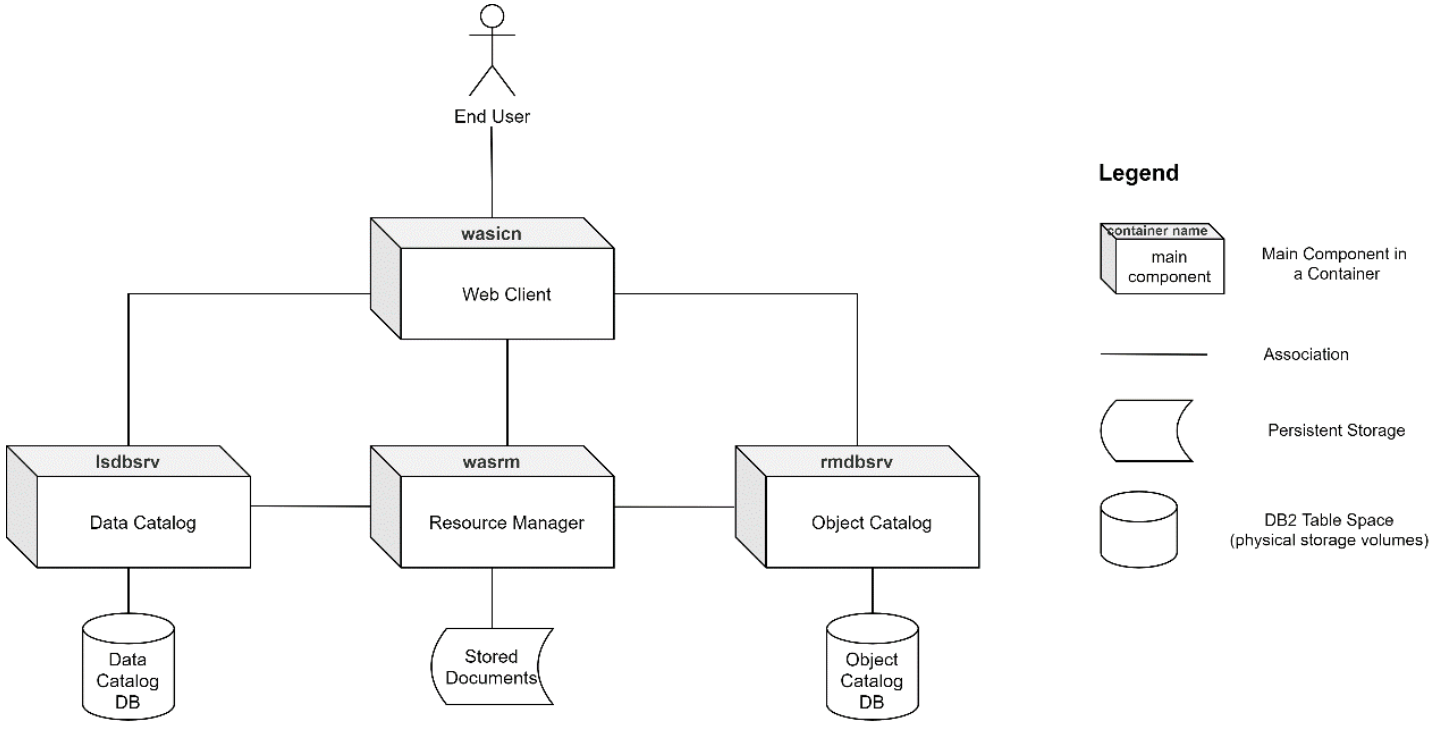
\includegraphics[width=\textwidth]{graphics/gang_system.png}
    \caption{Proof of Concept by Shao ~\cite{shao}}
    \label{fig:gang_system}
\end{figure}

\chapter{Concept}
\label{chap:concept}
The following chapter describes the applied changes to a containerized Enterprise Content Management application introduced by~\cite{shao} to be operated within a Kubernetes cluster.

\section{Implications of a Kubernetes Cluster}
After its donation to the open source community by Google Kubernetes has become the most popular orchestration platform to operate and deploy containerized applications with minimum manual effort.
The core concept of Kubernetes is the autonomous management of stateless applications which consist of identical, swappable and replaceable containers.
Enterprise Content Management systems and other real world applications typically need some kind of stateful service which is concerned with persistent data storage~\cite{KUB2}.
\\
\\
After analyzing the dependencies of the containerized ECM applications created by Shao~\cite{shao} we found out that the components can be divided in two web applications and two database applications.
Hence the web applications could be operated as stateless applications without further customization.
The considered containers are \textit{wasicn} with its web client component as well as \textit{wasrm} with the encompassed resource manager component.
The other components that are needed to construct a working ECM system are the data and the object catalog which both rely on databases to work properly.

\section{Aspired ECM System Topology}
The management of stateful applications like databases in a Kubernetes cluster is not trivial since it was designed to handle stateless workloads while keeping stateful components outside the managed cluster~\cite{KUB2}.
To pave the way to an operational ECM system we need to carefully examine how the state of the data as well as the object catalog can be preserved while being available to the cluster.
Additionally the initial Docker images provided by~\cite{shao} relied on the application data and executables to be locally present on the host machine.
There are two possibilities to achieve that each with its advantages and drawbacks:
\begin{itemize}
    \item[]{\textbf{Maintaining the State on the Host Node}\\
    To keep the state in filesystem of a host node it is crucial to upload the necessary data to that node on which the corresponding application will be operated.
    This approach implies that each potential node on which the corresponding application could be relocated by the \textit{Scheduling Layer} of the cluster has to contain the needed data.
    The data allocation on the computing nodes is illustrated in~\cref{fig:node_storage}.
    It shows that only nodes that have matching data can operate a certain application.
    In contrast to \textit{Node 2}, \textit{Node 1} and \textit{Node 3} contain the necessary \textit{Data} in their local filesystem and are able to host the application.
    Replicating the required data across all nodes of a large cluster leads to an overhead in storage allocation.
    By maintaining the data exclusively on dedicated nodes that operate only one specific application the flexibility and the availability of the whole system can be affected.
    In case of a failing node the \textit{Scheduling Layer} can not relocate the application autonomously on another node without applying procedures that ensure that the required data is present on the particular node.
    The biggest advantage of this procedure is the minimization of the latency of read and write operations all required data is already present on the local node.
    \begin{figure}[h]
    \centering
    
\includegraphics[width=0.95\textwidth]{graphics/node_storage.svg}
    \caption{Data Allocation in Local Filesystems of Host Servers in a Cluster}
    \label{fig:node_storage}
\end{figure}
    }
    \item[]{\textbf{Removing the State completely from the cluster}\\
    Relocating the state into an external storage service allows the \textit{Scheduling Layer} to scale or move the web applications without assumptions about the configuration of the computing nodes that form the cluster.
    The external service can be located on a separate Virtual Machine or on a physically separated host.
    Since the storage service is now moved to an external infrastructure it needs its own maintenance effort which can not be supervised through the \textit{Service Management Layer} of the cluster.
    Furthermore it can lead higher latencies of read and write operations due to the potential distance of the external infrastructure to the cluster.
    }
\end{itemize}
Given the complexity of setting up and managing stateful services in Kubernetes this thesis is restricted to stateless services.
Therefore the state is removed entirely from the cluster and an external Network File System server is utilized.
Further a stateful data service requires a much more complex cluster design and is easier to maintain and scale on its own.
Therefore the containerized applications can be scaled across the cluster independent of whether the volumes are mounted on a particular node or not.
The following~\cref{fig:high_level_topology} illustrates the initially aspired topology with all storage capacities transferred to the NFS server.
\begin{figure}[h]
    \centering
    
\includegraphics[width=0.95\textwidth]{graphics/high_level_topology.svg}
    \caption{Initial Cluster Topology}
    \label{fig:high_level_topology}
\end{figure}

\chapter{Prototype}
\label{chap:prototype}
In this chapter describes the prototypical implementation of the changes to the approach by Shao~\cite{shao} from the previous chapter to allow the operation within a Kubernetes cluster.

\section{Infrastructure}
The following prototype was developed, deployed and tested on the infrastructure of the Institute of Parallel and Distributed Systems at the University Stuttgart.
It consists of a Open Stack instance which manages the virtual machines running \textit{CentOS 8}\footnote{https://www.centos.org} that are used throughout this thesis.
To further simplify the development process and minimize the effort of setting up and managing a set of virtual machines as Kubernetes nodes this thesis relies on the KiND project.

\subsection{Kubernetes in Docker (KiND)}
The KiND Project uses multiple Docker containers to create a virtual Kubernetes cluster with multiple nodes.
It was created by the Kubernetes authors to enable a fast and straightforward way to test and verify cluster configurations on the local machine of a developer.
A KiND cluster consists of the following Docker images:
\begin{itemize}
    \item[]{\textbf{Base Image}\\
    This Image is based on Ubuntu and contains only the necessary dependencies for running nested containers, systemd and Kubernetes.
    Additionally it contains a custom entrypoint that allows to execute configurations before the container becomes available.}
    \item[]{\textbf{Node Image}\\
    This image is an extension of the Base Image and contains the tools required to operate and manage Kubernetes resources within a cluster.
    KiND aims to leverage existing tooling for Kubernetes to create a familiar environment for developers.}
\end{itemize}
Each node of a cluster runs its own Docker container which is identified through a Docker object label containing the cluster name and node id.
A KiND cluster consists of at least one control plane and one or many worker nodes.
The control plane handles incoming network traffic, storage mounts on the host machine and additional initial configurations of the cluster.
A worker node is equivalent to a compute node in a regular Kubernetes cluster~\cite{kind, KUB3}.

\subsection{Configuration of the Used Cluster}
To allow the external world to communicate with the applications inside a KiND cluster it is necessary to include a set \textit{extraPortMappings} in the cluster configuration file shown in~\cref{lst:cluster_config}.
\begin{Listing}
\begin{lstlisting}
kind: Cluster
apiVersion: kind.x-k8s.io/v1alpha4
name: ecm
nodes:
  - role: control-plane
    extraPortMappings:
      - containerPort: 30043
        hostPort: 9043
      - containerPort: 30044
        hostPort: 9044
      - containerPort: 30080
        hostPort: 9080
      - containerPort: 30081
        hostPort: 9081
      - containerPort: 30443
        hostPort: 9443
      - containerPort: 30444
        hostPort: 9444
  - role: worker
  - role: worker
  \end{lstlisting}
  \caption{KiND Cluster Configuration File}
  \label{lst:cluster_config}
\end{Listing}
Since Kubernetes only allows external ports to be in between $30000$ and $32767$ as well as the fact that KiND runs in Docker a workaround was needed to expose the expected ports on the host machine.
The workaround consists of \textit{nodePort} components inside the Kubernetes cluster that expose the ports of the application inside a pod which are then connected to the \textit{hostPort} of the \textit{controlPlane} container on the host server.
The applied workaround of the port mappings is shown in~\cref{fig:port_mapping}.
\begin{figure}[h]
    \centering
    
\includegraphics[width=0.8\textwidth]{graphics/port_mapping.svg}
    \caption{Workaround to Enable Incoming Traffic to the KiND Cluster}
    \label{fig:port_mapping}
\end{figure}

\section{Kubernetes Components}
To successfully run the aspired ECM system topology presented in~\cref{chap:concept} within a Kubernetes cluster the following components need to be utilized~\cite{KUB,KUB2,KUB3,KUB4}:
\begin{itemize}
    \item[]{\textbf{Namespaces}\\
    To enable the maintenance of multiple virtual clusters on a single physical cluster the concept of \textit{Namepaces} was introduced.
    It is especially helpful for managing the distribution of computing resource in large environments with multiple teams and projects.
    Thereby they allow the implementation of access control and resource quotas.
    Resource names must be unique within a \textit{Namespace} but not across different \textit{Namespaces}.
    Every cluster generates its own DNS space which is called \textit{cluster.local} and by placing an \textit{Service}-Object in a \textit{Namespace} the resulting fully qualified domain name (FQDN) will be \texttt{<object-name>.<namespace>.svc.cluster.local}.
    A \textit{Pod} inside the same \textit{Namespace} can connect to the \textit{Service} via its \texttt{<object-name>} but a \textit{Pod} from a different \textit{Namespace} needs the FQDN to establish a connection.
    }
    \item[]{\textbf{Pod}\\
    In Kubernetes a \textit{Pod} is the smallest unit that can be deployed and is a runtime isolation for a set of containers.
    The grouped containers are always deployed as a collective on the same host machine and the \textit{Scheduling Layer} strives to find a placement in the cluster which satisfies all constraints imposed by the incorporated containers.
    This pooling allows a fast exchange of information between each other by leveraging the file system, networking or inter process communication of the host.
    Additionally every \textit{Pod} has its own IP-address and thus a port range which is shared among all enclosed containers.
    Therefore it should be payed attention to port allocation at configuration time to prevent port conflicts.
    \textit{Pods} are designed to contain only a single instance of an application hence the \textit{Pod} should be replicated for scaling.
    Another key concept of Kubernetes is the the ephemerality of \textit{Pods} in their life cycle.
    That means that whenever a \textit{Pod} encounters an error the \textit{Pod} is not diagnosed and repaired but rather terminated and a new \textit{Pod} with identical properties is started.
    The same happens when a computation node fails: the \textit{Pods} on the node in question are not saved and moved to an available node but forgotten and a new set of \textit{Pods} is created.
    Even in the case of lightweight configuration changes the modification will not be passed to a running container instead the active \textit{Pod} will be terminated and a new one containing the changes will be spun up.
    To know if a container inside a \textit{Pod} is working properly Kubernetes runs a set of diagnostic functions on a container:
    \begin{itemize}
        \item[] {\textbf{ExecAction:} Performs a specified command inside the container and succeeds if the command terminates without an error.}
        \item[] {\textbf{TCPSocketAction:} Tries to open a TCP socket on a specified port of the \textit{Pods} IP-address and succeeds if a socket is opened.}
        \item[] {\textbf{HTTPGetAction:} Sends a HTTP \texttt{GET} request to a specified port and route on the \textit{Pods} IP-address and succeeds if the status code of the response is between \texttt{200} and \texttt{400}.}
    \end{itemize}
    Kubernetes provides the previously introduced functions to monitor the following conditions a \textit{Pod} could encounter during its life cycle:
    \begin{itemize}
        \item[] {\textbf{Startup:} Monitors if the application inside a container successfully launched during the start up phase of the \textit{Pod}.
        The following conditions are only evaluated if the Startup was successful.
        It is especially helpful for large and complex applications that need a certain time span to become available for service.
        }
        \item[] {\textbf{Readiness:} Evaluates whether the container is able to respond to requests.
        If the probe fails Kubernetes prevents incoming traffic to be passed to the \textit{Pod} by removing its IP-address from the \textit{Endpoint} objects of all \textit{Services} that reference the \textit{Pod}.
        }
        \item[] {\textbf{Liveness:} Continuously checks whether a container is in a functional state to process incoming requests.
        This probe should be used if an application has a strong dependency on a external back-end service to prevent information loss.
        }
    \end{itemize}
    If the \textit{Startup} and \textit{Liveness} probes fail Kubernetes autonomously terminates the \textit{Pod} and launches a new one.
    The termination happens gracefully since \textit{Pods} are distributed processes running distributed within a cluster.
    Abruptly killing processes without a cleanup phase can leave corrupted data and open database connections behind.
    To prevent those undesirable residuals, clean up commands can be passed through a specified \textit{postStop} hook.
    It is executed after the termination signal reached the \textit{Pod} and before the \texttt{TERM} signal is passed to the process with the id $1$ inside each container.
    }
    \item[]{\textbf{ReplicaSets}\\
    A \textit{ReplicaSet} takes care of maintaining a specified number of identical active \textit{Pods} at any given point in time.
    It contains a selector that identifies which \textit{Pods} should be monitored, a count of how many \textit{Pods} should be running simultaneously and a template which describes the properties newly generated \textit{Pods} should comply with.
    It is considered a best practice to only interact directly with \textit{ReplicaSets} when dealing with complex deployment scenarios.
    In regular circumstances it should be sufficient to utilize \textit{Deployments} to manage the deployed \textit{Pods}.
    }
    \item[]{\textbf{Deployments}\\
    The update and start of applications inside a cluster in a declarative way is performed through \textit{Deployment} configuration files.
    They serve as a blueprint of the service an application should provide.
    A \textit{Deployment} contains the desired state of an application in regard to the number of pods, which image should be used for the containers inside the \textit{Pods}, the assignment of network ports and information about how to perform rolling updates.
    To accomplish a successful rolling update by deploying a new version of the image of an application the updated \textit{Deployments} file is resubmitted to the Kubernetes API server.
    It detects a new desired state in the cluster and creates a new \textit{ReplicaSet} for the \textit{Pods} containing the updated image.
    So now the cluster contains a new and an old \textit{ReplicaSet} and each time a new \textit{Pod} with the updated image is launched a running \textit{Pod} containing the deprecated image is terminated.
    This procedure allows a smooth update process with minimized downtime.
    After performing a rolling update by default the previous $10$ outdated \textit{ReplicaSets} containing their whole configuration are retained in the cluster without managing active \textit{Pods}.
    Hence a rollback is essentially a rolling update the other way around to a desired previous version of the application.
    Additionally the prior described \textit{Startup-}, \textit{Readiness} and \textit{Liveness}-Probes need to be specified within the \textit{Deployments} files.
    \cref{fig:kub_components} illustrates that \textit{Deployments} are controlling \textit{ReplicaSets}, and \textit{ReplicaSets} are managing \textit{Pods}.
    }
    \item[]{\textbf{PersistentVolumes}\\
    \textit{Pods} in a cluster are intended to be stateless but sometimes external storage needs to be mapped onto the cluster to provide data and storage capacity for the running applications.
    This component was introduced to abstract the usage of storage from its provision since managing storage differs from managing computing resources. 
    \textit{PersistentVolumes} differ in life cycle from \textit{Pods} and contain the information to use NFS or storage options provided by cloud vendors.
    They come in two different forms:
    \begin{itemize}
        \item[] {\textbf{Static: }A fixed set of \textit{PersistentVolumes} is manually created at configuration time and can be consumed by applications within the cluster.}
        \item[] {\textbf{Dynamic: }Kubernetes autonomously allocates \textit{PeristentVolumes} at run time based on a \textit{StorageClass} defined during configuration time.
        This happens if and only if a matching \textit{PersistentVolumeClaim} exists.
        By defining the \textit{StorageClass} as an empty string in a \textit{PersistentVolumeClaim} the dynamic provision is disabled.}
    \end{itemize}
    }
    \item[]{\textbf{Persistent Volume Claim}\\
    The \textit{Persistent Volume Claim} authorizes the applications inside a \textit{Pod} to access the specified \textit{PersistentVolume}.
    The configuration file contains information about the needed storage capacity, access mode, \textit{StorageClass} etc.
    It gets bound to a \textit{PeristentVolume} by Kubernetes on a one-on-one basis as soon as the specified conditions are satisfied.
    Otherwise the claim will remain unbound until new resources are added to the cluster or already utilized are freed.
    Depending on the storage provider a \textit{PersistentVolumeClaim} is able to consume storage with different access modes:
    \begin{itemize}
        \item[] {\textbf{ReadWriteOnce:} One node can exclusively write on this volume.}
        \item[] {\textbf{ReadOnlyMany:} Many nodes can read jointly from this volume.}
        \item[] {\textbf{ReadWriteMany:} Many nodes can read from as well as write to this volume.}
    \end{itemize}
    Network File Storage supports all previously discussed access modes.
    }
    \item[]{\textbf{Storage Classes}\\
    This component allows to specify classes of provided storage which may differ in the enforced policies by the storage service administration like quality-of-service, backup etc.
    }
    \item[]{\textbf{Service}\\
    Because of the dynamic nature of scaling and locating \textit{Pods} throughout a Kubernetes cluster it is not feasible to use the IP-address of a \textit{Pod} to communicate with the applications it contains.
    \textit{Services} were introduced to provide a stable and reliable networking interface for a set of ephemeral \textit{Pods}.
    It exposes a defined host name and ports that are immutable at run time.
    \textit{Pods} and \textit{Services} have a one-to-one correspondence and are mapped through the \textit{app} selector label.
    By omitting the selector label the corresponding \textit{Service} won't create an \textit{Endpoint} object.
    This is useful to incorporate applications that operate on an external host like database applications.
    }
    \item[]{\textbf{Nodeport}\\
    In Kubernetes the \textit{Pods} within the cluster are not reachable from the outside.
    This component is a special type of \textit{Service} which allows to reach the internal IP-space of the cluster from external applications.
    Kubernetes either autonomously assigns an access port or applies a specified port in the range of $30000$ and $32767$.
    \textit{Nodeports} are not able to manage incoming traffic like a \textit{Load Balancer} component and should therefore not be used in production systems.
    Since this thesis aims to investigate whether ECM systems can be managed by Kubernetes at all the aspect of load balancing is out of scope but is considered in the companion master thesis~\cite{pascal2021}.
    }
    \item[]{\textbf{Endpoints}\\
    \textit{Endpoints} are dynamic objects that contain all the available \textit{Pods} and their IP-addresses and ports.
    Before directing traffic to \textit{Pods} the corresponding \textit{Service} queries the \textit{Endpoints} object to get the addresses of currently available \textit{Pods} and then chooses one to direct the request to.
    }
\end{itemize}

\cref{fig:kub_components} illustrates the previously presented components and its interactions inside a cluster to maintain its specified desired state.

\begin{figure}[h]
    \centering
    
\includegraphics[width=0.8\textwidth]{graphics/kub_components.svg}
    \caption{The Interactions of the Components Inside a Kubernetes Cluster~\cite{KUB4}}
    \label{fig:kub_components}
\end{figure}

\section{Initially Aspired System Topology}
\label{sec:init_topo}
The following~\cref{fig:init_topology} shows the previously presented components and its role to implement a scalable Enterprise Content Management system based on the concept introduced in~\cref{chap:concept}.
\\
\\
The overall System is split in two parts the Kubernetes cluster and a NFS server which holds all the data needed to operate the applications inside the cluster.
The vertical dashed lines indicate the separation of the individual ECM applications.
Each application utilizes a \textit{PersistentVolume} with a corresponding \textit{PersistentVolumeClaim} to either load needed application data or read from or write to database files.
The \textit{Resource Manager} application requires two JDBC connections to the \textit{Object Catalog} and \textit{Data Catalog} as well as an external connection for administration.
The \textit{Web Client} portal application only requires an internal connection to the \textit{Object Catalog}, an internal connection to the \textit{Resource Manager} and an external to provide user access.
External connections are implemented through \textit{Nodeports} to enable user interaction.

\begin{figure}[h]
    \centering
    
\includegraphics[width=0.95\textwidth]{graphics/initial_topology.svg}
    \caption{Initial Topology of the ECM System Inside a Kubernetes Cluster}
    \label{fig:init_topology}
\end{figure}

\section{Refactored ECM System Topology}
The initially aspired system topology described in~\cref{sec:init_topo} turned out to be brittle when put under load.
During functional tests it was discovered that the topology design required a refactoring as the stateful database service was very unstable and unreliable.
It could sometimes handle manual queries as well as file uploads and sometimes the databases would crash for no obvious reason.
Following investigations showed that running DB2 instances on NFS storage was the source of the occurring issues.
\\
\\
To enhance the prototype stability and therefore availability we decided to remove the stateful database services from the cluster and operate it as \textit{Docker} containers on a different host server.
This decision resulted in removing the \textit{Deployment}, \textit{PersistentVolume} and \textit{PersistentVolumeClaim} components and adding a \textit{Endpoints} component for both the \textit{Object Catalog} and the \textit{Data Catalog}.
Besides that a new Docker image was created which contains all essential files of the \textit{Resource Manager} and \textit{Web Client} applications such that external file mounts are avoided.
Hence the \textit{Persistent Volume} and \textit{Persistent Volume Claim} component were removed from the topology.
The new image incorporates both applications and the startup of the separate systems is enforced through various configurations when starting the corresponding container.
The following~\cref{fig:improv_topology} illustrates the refactored topology to prevent the previously discussed challenges of the initial implementation.

\begin{figure}[h]
    \centering
    
\includegraphics[width=0.7\textwidth]{graphics/improved_topology.svg}
    \caption{Improved Topology of the ECM System Inside a Kubernetes Cluster}
    \label{fig:improv_topology}
\end{figure}

\section{Implementation Details of the Kubernetes Components}
The following section describes the configuration of the components of a Enterprise Content Management system within a Kubernetes cluster.
It describes the implementation by means of source code with a detailed explanation of the design decisions made.

\subsection{Data Catalog and Object Catalog}
Because the \textit{Data Catalog} and \textit{Object Catalog} are relocated to an external server outside the cluster they require means to communicate with the applications left inside the cluster.
To achieve this a \textit{Service} without the app selector and a manually configured \textit{Endpoint} object is necessary.
Since the configuration files of both components have only minor disparities only the \textit{Data Catalog} configuration is displayed. 
\begin{itemize}
    \item[]{\textbf{Service}\\
    The \textit{Service} configuration file is described in~\cref{lst:service_lsdb_config}.
    The specified \textit{port} in the \textit{spec} section has to correspond to the port exposed within the cluster whereas the \textit{targetPort} needs to correspond with the port configured in the \textit{Endpoint} object.
    The \textit{Service} configuration of the \textit{Object Catalog} component is identical except for the \textit{port} and \textit{targetPort} number which is $50001$.
\begin{Listing}[h]
\begin{lstlisting}
kind: Service
apiVersion: v1
metadata:
  name: icm86-ls
  namespace: ecm
spec:
  ports:
    - port: 50000
      targetPort: 50000
\end{lstlisting}
\caption{Data Catalog Database~\textit{Service} Configuration File}
\label{lst:service_lsdb_config}
\end{Listing}
    }
    \item[]{\textbf{Endpoint}\\
    The \textit{Endpoint} configuration file is described in~\cref{lst:endpoint_lsdb_config}.
    The described \textit{port} corresponds directly to the exposed port of the external data source which is reachable through the specified IP-address.
    The configuration file of the \textit{Object Catalog} \textit{Endpoint} is identical except for the \textit{port} number which is $50001$
    
\begin{Listing}[h]
\begin{lstlisting}
kind: Endpoints
apiVersion: v1
metadata:
  name: icm86-ls
  namespace: ecm
subsets:
  - addresses:
      - ip: 192.168.221.148
    ports:
      - port: 50000
\end{lstlisting}
\caption{Data Catalog Database~\textit{Endpoint} Configuration File}
\label{lst:endpoint_lsdb_config}
\end{Listing}
    }
\end{itemize}

\subsection{Resource Manager Application and Content Navigator}
Since the configuration files for the components of the \textit{Resource Manager} and \textit{Web Client} applications are almost identical just the \textit{Resource Manager} is considered in the following section.
As displayed in~\cref{fig:improv_topology} both applications depend of the following Kubernetes components:
\begin{itemize}
    \item[]{\textbf{Nodeport}\\
    The \textit{Nodeport} configuration file is described in~\cref{lst:nodeport_config}.
    Because we want Kubernetes to take as much work from our hands as possible the \textit{Nodeport} configurations of components inside the cluster all contain the app selector in the \textit{spec} field.
    Therefore we don't need to worry about \textit{Endpoints} objects.
    The defined \textit{nodePorts} inside the \textit{ports} specification exposes the corresponding \textit{ports} and \textit{targetPorts} of the application inside the \textit{Pods}.
    Since our cluster resides in an emulated environment using Docker containers the exposed ports need to be looped through the Docker network layer to be reachable from outside the \textit{Control Plane} container.
    \cref{fig:port_mapping} illustrates the applied port mappings.
\begin{Listing}[h]
\begin{lstlisting}
kind: Service
apiVersion: v1
metadata:
  name: icm86-rmapp-nodeport
  namespace: ecm
spec:
  type: NodePort
  selector:
    app: icm86-rmapp
  ports:
    - name: icm86-rmapp-websphere-admin-port
      port: 9043
      targetPort: 9043
      nodePort: 30044
      protocol: TCP
    - name: icm86-rmapp-insecure-application-port
      port: 9080
      targetPort: 9080
      nodePort: 30080
      protocol: TCP
    - name: icm86-rmapp-secure-application-port
      port: 9443
      targetPort: 9443
      nodePort: 30443
      protocol: TCP
\end{lstlisting}
\caption{Resource Manager Application~\textit{Nodeport} Configuration File}
\label{lst:nodeport_config}
\end{Listing}
    }
    \item[]{\textbf{Service}\\
    The \textit{Service} configuration contains only minor differences compared to the \textit{Nodeport} configuration described in~\cref{lst:nodeport_config}.
    It does not contain a \texttt{spec.type} attribute nor a \texttt{spec.ports.nodePort} attribute in each port definition.
    This \textit{Service} handles the communication between \textit{Web Client} and \textit{Resource Manager}.
    }
    \item[]{\textbf{Deployment}\\
    The \textit{Deployment} configuration file is described in~\cref{lst:deployment_config}.
    It contains all information needed to operate the applications within a cluster.
    For the Minimum Viable Prototype implemented during this thesis the number of \texttt{spec.replicas} was set to $1$.
    The entry \texttt{spec.selector.matchLabels.app} sets a label to describe with which \textit{Pods} the \textit{Deployment} is associated.
    The following section \texttt{spec.template} contains all information for the \textit{ReplicaSet} to generate new \textit{Pods} if necessary.
    \texttt{spec.template.metadata} defines the label inside the cluster which is used by \textit{Services} to direct traffic to the deployed \textit{Pods}
    The next section defined in \texttt{spec.template.spec.containers} specifies the structure of the launched \textit{Containers} inside the \textit{Pod} and details concerned with its life cycle.
    Following the generation of the \textit{Container} based on the chosen image and the exposed ports the specified command is executed.
    The \texttt{spec.template.spec.containers.command} runs the \textit{entrypoint} script inside the root directory of the image which is described in~\cref{lst:entrypoint}.
    Simultaneously when starting the \texttt{command} the \texttt{startupProbe} is launched.
    It continuously evaluates whether a TCP connection can be established with port $9443$.
    The configuration of this probe allows a $15$ minute time frame for the application to start before terminating the \textit{Pod}.
    The port $9443$ was selected because the main application can be reached that way so as soon as a connection would succeed the \textit{Ressource Manager Application} could be used.
    The large time frame is chosen due to long start up phase of the \textit{WebSphere Application Server}.
    Due to design decisions of the Docker image the \textit{Container} has to be kept running.
    Therefore Kubernetes is not able to know whether the application inside the \textit{container} was still in a healthy state.
    As a countermeasure the \texttt{livenessProbe} and \texttt{readinessProbe} are utilized based on the same assumptions regarding the port as the \texttt{startupProbe}.
    The first reports to Kubernetes after $3$ failed connection attempts that the \textit{Pod} has to be restarted.
    The second probe instructs the \textit{Service} to stop directing traffic to the \textit{Pod} after $1$ failed connection attempt.
    After a \textit{Pod} is flagged as failed or the \textit{Pod} gets terminated due to scaling requirements \texttt{spec.template.spec.containers.lifecycle.preStop} is executed.
    This command allows a graceful shutdown of the \textit{Websphere Application Server} inside the \textit{Pod} within the default time frame of $30$ seconds to prevent eventual resource leaks.
\begin{Listing}[h]
\begin{lstlisting}
kind: Deployment
apiVersion: apps/v1
metadata:
  name: icm86-rmapp
  namespace: ecm
spec:
  replicas: 1
  selector:
    matchLabels:
      app: icm86-rmapp
  template:
    metadata:
      labels:
        app: icm86-rmapp
    spec:
      containers:
      - name: icm86-rmapp
        image: ecmdocker.novalocal:5043/ipvs-as/icm86/cm8-rmapp:v1.2.5
        ports:
        - containerPort: 80
        - containerPort: 9043
        - containerPort: 9080
        - containerPort: 9443
        command:
        - "/root/entrypoint.sh"
        startupProbe:
          failureThreshold: 30
          periodSeconds: 20
          timeoutSeconds: 10
          tcpSocket:
            port: 9443
        livenessProbe:
          periodSeconds: 5
          timeoutSeconds: 2
          successThreshold: 1
          failureThreshold: 3
          tcpSocket:
            port: 9443
        readinessProbe:
          periodSeconds: 5
          timeoutSeconds: 2
          successThreshold: 1
          failureThreshold: 1
          tcpSocket:
            port: 9443
        lifecycle:
          preStop:
            exec:
              command:
              - "/bin/bash -c"
              - "/opt/IBM/WebSphere/AppServer/profiles/icm86AppProfile/bin/stopServer.sh 
                server1 -profileName icm86AppProfile -username wasadmin -password passw0rd"
\end{lstlisting}
\caption{Resource Manager Application~\textit{Deployment} Configuration File}
\label{lst:deployment_config}
\end{Listing}
    \begin{itemize}
        \item[] {\textbf{Entrypoint Script}\\
        To successfully start the Resource Manager and the Content Navigator applications the following \textit{entrypoint.sh} script is run during setup time.
        The developed script is displayed in~\cref{lst:entrypoint}.
        At first it is enforced through \texttt{pipefail} that the whole script should exit with a non-zero status code if any command or pipe exits with a non-zero status code.
        Subsequently the start script for the \textit{WebSphere Application Server} is called.
        After a successful start the script maps the logs of the application to \textit{STDOUT} using the \texttt{tail} command.
        The final step serves two purposes, at first it allows to inspect the logs from the outside of the \textit{Pod} by using \texttt{kubectl logs}.
        Secondly it prevents the container from exiting and thus terminating the whole \textit{Pod}.
        This procedure is necessary because the initially generated Docker image was operated in \textit{interactive} mode.
        This means that the \textit{Docker Demon} keeps the \textit{STDIN} open even if the container is running in \textit{detached} mode.
        Since Kubernetes \textit{Deployments} do not support an \textit{interactive} mode this workaround had to be implemented.
\begin{Listing}[h]
\begin{lstlisting}
#!/usr/bin/env bash
set -Eeuo pipefail

echo -e "\n start the ICN-WAS server in the foreground "
/root/icmStartWas.sh

echo -e "ICN-WAS instance ready to go; tailing the sysout log file ..."
/usr/bin/tail -n 100 -F /opt/IBM/WebSphere/AppServer/profiles/icm86AppProfile/logs/server1/rm/icmrm/icmrm.logfile
\end{lstlisting}
\caption{Resource Manager Application~\textit{Deployment} \textit{entrypoint.sh} script}
\label{lst:entrypoint}
\end{Listing}
        }
    \end{itemize}
    }
\end{itemize}

\section{Source Code}
The source code and image developed during this master thesis can be obtained from an internal repository resp. registry of the Institute of Parallel and Distributed Systems at the University Stuttgart.
It includes the configuration files for the Kubernetes cluster as well as scripts to install all required dependencies, setup the environment and start all cluster components except the required \textit{Docker} image.
The following steps work only within the environment of the university.
\\
\\
To install all dependencies and load the Docker images from the internal registry simply run \texttt{./runSetupJobs.sh} in the root directory of the repository.
It is important to mention that the required image to start the \textit{Pods} inside the \textit{KiND} cluster needs to be loaded in the Docker instance of the host beforehand.
After all dependencies are available the \texttt{./start.sh} script can be executed which goes through following steps:
\begin{enumerate}
    \item Delete any old \textit{KiND} cluster with the name \textit{kind-ecm}
    \item Create a new cluster based on the configuration file displayed in~\cref{lst:cluster_config}
    \item Set the \textit{kubectl} context to the newly generated cluster
    \item Load the required Docker images into the cluster
    \item Instruct \texttt{kubectl} to create all required components
\end{enumerate}
Since loading all Docker images into \textit{KiND} can take a long time the additional script \texttt{repopulate.sh} was created.
It allows to delete all components inside the cluster and recreate them based on new configuration files without deleting the cluster and reloading all Docker images.

\chapter{Conclusion and Outlook}
\label{chap:zusfas}
This thesis demonstrates that the approach by Shao~\cite{shao} can be operated properly on a \textit{Docker} based container environment but it was not possible to apply a one to one porting into a Kubernetes cluster.
The cluster needs to be further enhanced to handle stateful database services in an automated manner by leveraging Kubernetes technology.
\\
\\
This work evaluates two approaches of operating stateful applications inside Kubernetes.
Based on this investigation the first concept is proposed and implemented in the form of a prototype.
While conducting reliability tests it turned out that the developed solutions of running the \textit{Data Catalog} and \textit{Object Catalog} of the ECM system could not guarantee a stable and reliable operation inside the cluster. 
The objective of managing stateful database applications inside a Kubernetes cluster poses as a serious challenge and requires a much more complex deployment design.
This is mainly because Kubernetes was designed to autonomously manage stateless workloads.
Therefore the stateful components were removed and managed on an external infrastructure.
In the end the effort was split in two phases: primarily focus on implementing the stateless components and secondarily further improve the initial approach to handle stateful components.
Given the time constraints for this thesis and the complexity of the task the stateful databases services are left on the external docker environment.
Additionally the stateless applications which stayed inside the cluster required the creation of a new Docker image which eliminated the need of external data sources mounted into the \textit{Pods}.
\\
\\
Future work might improve the developed prototype through investigating the areas of load balancing, dynamic scaling and security in Kubernetes clusters.

\printbibliography

All links were last followed on August 30, 2021.

\appendix

\pagestyle{empty}
\renewcommand*{\chapterpagestyle}{empty}
\Versicherung
\end{document}
